% ----------------------------------------------------------------------
%
%                            TFMTesis.tex
%
%----------------------------------------------------------------------
%
% Este fichero contiene el "documento maestro" del documento. Lo único
% que hace es configurar el entorno LaTeX e incluir los ficheros .tex
% que contienen cada sección.
%
%----------------------------------------------------------------------
%
% Los ficheros necesarios para este documento son:
%
%       TeXiS/* : ficheros de la plantilla TeXiS.
%       Cascaras/* : ficheros con las partes del documento que no
%          son capítulos ni apéndices (portada, agradecimientos, etc.)
%       Capitulos/*.tex : capítulos de la tesis
%       Apendices/*.tex: apéndices de la tesis
%       constantes.tex: constantes LaTeX
%       config.tex : configuración de la "compilación" del documento
%       guionado.tex : palabras con guiones
%
% Para la bibliografía, además, se necesitan:
%
%       *.bib : ficheros con la información de las referencias
%
% ---------------------------------------------------------------------

\documentclass[11pt,a4paper,twoside]{book}

%
% Definimos  el   comando  \compilaCapitulo,  que   luego  se  utiliza
% (opcionalmente) en config.tex. Quedaría  mejor si también se definiera
% en  ese fichero,  pero por  el modo  en el  que funciona  eso  no es
% posible. Puedes consultar la documentación de ese fichero para tener
% más  información. Definimos también  \compilaApendice, que  tiene el
% mismo  cometido, pero  que se  utiliza para  compilar  únicamente un
% apéndice.
%
%
% Si  queremos   compilar  solo   una  parte  del   documento  podemos
% especificar mediante  \includeonly{...} qué ficheros  son los únicos
% que queremos  que se incluyan.  Esto  es útil por  ejemplo para sólo
% compilar un capítulo.
%
% El problema es que todos aquellos  ficheros que NO estén en la lista
% NO   se  incluirán...  y   eso  también   afecta  a   ficheros  de
% la plantilla...
%
% Total,  que definimos  una constante  con los  ficheros  que siempre
% vamos a querer compilar  (aquellos relacionados con configuración) y
% luego definimos \compilaCapitulo.
\newcommand{\ficherosBasicosTeXiS}{%
TeXiS/TeXiS_pream,TeXiS/TeXiS_cab,TeXiS/TeXiS_bib,TeXiS/TeXiS_cover%
}
\newcommand{\ficherosBasicosTexto}{%
constantes,guionado,Cascaras/bibliografia,config%
}
\newcommand{\compilaCapitulo}[1]{%
\includeonly{\ficherosBasicosTeXiS,\ficherosBasicosTexto,Capitulos/#1}%
}

\newcommand{\compilaApendice}[1]{%
\includeonly{\ficherosBasicosTeXiS,\ficherosBasicosTexto,Apendices/#1}%
}

%- - - - - - - - - - - - - - - - - - - - - - - - - - - - - - - - - - -
%            Preámbulo del documento. Configuraciones varias
%- - - - - - - - - - - - - - - - - - - - - - - - - - - - - - - - - - -

% Define  el  tipo  de  compilación que  estamos  haciendo.   Contiene
% definiciones  de  constantes que  cambian  el  comportamiento de  la
% compilación. Debe incluirse antes del paquete TeXiS/TeXiS.sty
%---------------------------------------------------------------------
%
%                          config.tex
%
%---------------------------------------------------------------------
%
% Contiene la  definición de constantes  que determinan el modo  en el
% que se compilará el documento.
%
%---------------------------------------------------------------------
%
% En concreto, podemos  indicar si queremos "modo release",  en el que
% no  aparecerán  los  comentarios  (creados  mediante  \com{Texto}  o
% \comp{Texto}) ni los "por  hacer" (creados mediante \todo{Texto}), y
% sí aparecerán los índices. El modo "debug" (o mejor dicho en modo no
% "release" muestra los índices  (construirlos lleva tiempo y son poco
% útiles  salvo  para   la  versión  final),  pero  sí   el  resto  de
% anotaciones.
%
% Si se compila con LaTeX (no  con pdflatex) en modo Debug, también se
% muestran en una esquina de cada página las entradas (en el índice de
% palabras) que referencian  a dicha página (consulta TeXiS_pream.tex,
% en la parte referente a show).
%
% El soporte para  el índice de palabras en  TeXiS es embrionario, por
% lo  que no  asumas que  esto funcionará  correctamente.  Consulta la
% documentación al respecto en TeXiS_pream.tex.
%
%
% También  aquí configuramos  si queremos  o  no que  se incluyan  los
% acrónimos  en el  documento final  en la  versión release.  Para eso
% define (o no) la constante \acronimosEnRelease.
%
% Utilizando \compilaCapitulo{nombre}  podemos también especificar qué
% capítulo(s) queremos que se compilen. Si no se pone nada, se compila
% el documento  completo.  Si se pone, por  ejemplo, 01Introduccion se
% compilará únicamente el fichero Capitulos/01Introduccion.tex
%
% Para compilar varios  capítulos, se separan sus nombres  con comas y
% no se ponen espacios de separación.
%
% En realidad  la macro \compilaCapitulo  está definida en  el fichero
% principal tesis.tex.
%
%---------------------------------------------------------------------


% Comentar la línea si no se compila en modo release.
% TeXiS hará el resto.
% ¡¡¡Si cambias esto, haz un make clean antes de recompilar!!!
\def\release{1}


% Descomentar la linea si se quieren incluir los
% acrónimos en modo release (en modo debug
% no se incluirán nunca).
% ¡¡¡Si cambias esto, haz un make clean antes de recompilar!!!
%\def\acronimosEnRelease{1}


% Descomentar la línea para establecer el capítulo que queremos
% compilar

% \compilaCapitulo{01Introduccion}
% \compilaCapitulo{02EstructuraYGeneracion}
% \compilaCapitulo{03Edicion}
% \compilaCapitulo{04Imagenes}
% \compilaCapitulo{05Bibliografia}
% \compilaCapitulo{06Makefile}

% \compilaApendice{01AsiSeHizo}

% Variable local para emacs, para  que encuentre el fichero maestro de
% compilación y funcionen mejor algunas teclas rápidas de AucTeX
%%%
%%% Local Variables:
%%% mode: latex
%%% TeX-master: "./Tesis.tex"
%%% End:


% Paquete de la plantilla
\usepackage{TeXiS/TeXiS}

% Incluimos el fichero con comandos de constantes
%---------------------------------------------------------------------
%
%                          constantes.tex
%
%---------------------------------------------------------------------
%
% Fichero que  declara nuevos comandos LaTeX  sencillos realizados por
% comodidad en la escritura de determinadas palabras
%
%---------------------------------------------------------------------

%%%%%%%%%%%%%%%%%%%%%%%%%%%%%%%%%%%%%%%%%%%%%%%%%%%%%%%%%%%%%%%%%%%%%%
% Comando: 
%
%       \titulo
%
% Resultado: 
%
% Escribe el título del documento.
%%%%%%%%%%%%%%%%%%%%%%%%%%%%%%%%%%%%%%%%%%%%%%%%%%%%%%%%%%%%%%%%%%%%%%
\def\titulo{Chatbot para la recuperación de
	información personal}

%%%%%%%%%%%%%%%%%%%%%%%%%%%%%%%%%%%%%%%%%%%%%%%%%%%%%%%%%%%%%%%%%%%%%%
% Comando: 
%
%       \autor
%
% Resultado: 
%
% Escribe el autor del documento.
%%%%%%%%%%%%%%%%%%%%%%%%%%%%%%%%%%%%%%%%%%%%%%%%%%%%%%%%%%%%%%%%%%%%%%
\def\autor{Luc\'ia Latorre Magaz}

% Variable local para emacs, para  que encuentre el fichero maestro de
% compilación y funcionen mejor algunas teclas rápidas de AucTeX

%%%
%%% Local Variables:
%%% mode: latex
%%% TeX-master: "tesis.tex"
%%% End:


% Sacamos en el log de la compilación el copyright
%\typeout{Copyright Marco Antonio and Pedro Pablo Gomez Martin}

%
% "Metadatos" para el PDF
%
\ifpdf\hypersetup{%
    pdftitle = {\titulo},
    pdfsubject = {Plantilla de Tesis},
    pdfkeywords = {Plantilla, LaTeX, tesis, trabajo de
      investigación, trabajo de Master},
    pdfauthor = {\textcopyright\ \autor},
    pdfcreator = {\LaTeX\ con el paquete \flqq hyperref\frqq},
    pdfproducer = {pdfeTeX-0.\the\pdftexversion\pdftexrevision},
    }
    \pdfinfo{/CreationDate (\today)}
\fi


%- - - - - - - - - - - - - - - - - - - - - - - - - - - - - - - - - - -
%                        Documento
%- - - - - - - - - - - - - - - - - - - - - - - - - - - - - - - - - - -
\begin{document}

% Incluimos el  fichero de definición de guionado  de algunas palabras
% que LaTeX no ha dividido como debería
%----------------------------------------------------------------
%
%                          guionado.tex
%
%----------------------------------------------------------------
%
% Fichero con algunas divisiones de palabras que LaTeX no
% hace correctamente si no se le da alguna ayuda.
%
%----------------------------------------------------------------

\hyphenation{
% a
abs-trac-to
abs-trac-tos
abs-trac-ta
abs-trac-tas
ac-tua-do-res
a-gra-de-ci-mien-tos
ana-li-za-dor
an-te-rio-res
an-te-rior-men-te
apa-rien-cia
a-pro-pia-do
a-pro-pia-dos
a-pro-pia-da
a-pro-pia-das
a-pro-ve-cha-mien-to
a-que-llo
a-que-llos
a-que-lla
a-que-llas
a-sig-na-tu-ra
a-sig-na-tu-ras
a-so-cia-da
a-so-cia-das
a-so-cia-do
a-so-cia-dos
au-to-ma-ti-za-do
% b
batch
bi-blio-gra-fía
bi-blio-grá-fi-cas
bien
bo-rra-dor
boo-l-ean-expr
% c
ca-be-ce-ra
call-me-thod-ins-truc-tion
cas-te-lla-no
cir-cuns-tan-cia
cir-cuns-tan-cias
co-he-ren-te
co-he-ren-tes
co-he-ren-cia
co-li-bri
co-men-ta-rio
co-mer-cia-les
co-no-ci-mien-to
cons-cien-te
con-si-de-ra-ba
con-si-de-ra-mos
con-si-de-rar-se
cons-tan-te
cons-trucción
cons-tru-ye
cons-tru-ir-se
con-tro-le
co-rrec-ta-men-te
co-rres-pon-den
co-rres-pon-dien-te
co-rres-pon-dien-tes
co-ti-dia-na
co-ti-dia-no
crean
cris-ta-li-zan
cu-rri-cu-la
cu-rri-cu-lum
cu-rri-cu-lar
cu-rri-cu-la-res
% d
de-di-ca-do
de-di-ca-dos
de-di-ca-da
de-di-ca-das
de-rro-te-ro
de-rro-te-ros
de-sa-rro-llo
de-sa-rro-llos
de-sa-rro-lla-do
de-sa-rro-lla-dos
de-sa-rro-lla-da
de-sa-rro-lla-das
de-sa-rro-lla-dor
de-sa-rro-llar
des-cri-bi-re-mos
des-crip-ción
des-crip-cio-nes
des-cri-to
des-pués
de-ta-lla-do
de-ta-lla-dos
de-ta-lla-da
de-ta-lla-das
di-a-gra-ma
di-a-gra-mas
di-se-ños
dis-po-ner
dis-po-ni-bi-li-dad
do-cu-men-ta-da
do-cu-men-to
do-cu-men-tos
% e
edi-ta-do
e-du-ca-ti-vo
e-du-ca-ti-vos
e-du-ca-ti-va
e-du-ca-ti-vas
e-la-bo-ra-do
e-la-bo-ra-dos
e-la-bo-ra-da
e-la-bo-ra-das
es-co-llo
es-co-llos
es-tu-dia-do
es-tu-dia-dos
es-tu-dia-da
es-tu-dia-das
es-tu-dian-te
e-va-lua-cio-nes
e-va-lua-do-res
exis-ten-tes
exhaus-ti-va
ex-pe-rien-cia
ex-pe-rien-cias
% f
for-ma-li-za-do
% g
ge-ne-ra-ción
ge-ne-ra-dor
ge-ne-ra-do-res
ge-ne-ran
% h
he-rra-mien-ta
he-rra-mien-tas
% i
i-dio-ma
i-dio-mas
im-pres-cin-di-ble
im-pres-cin-di-bles
in-de-xa-do
in-de-xa-dos
in-de-xa-da
in-de-xa-das
in-di-vi-dual
in-fe-ren-cia
in-fe-ren-cias
in-for-ma-ti-ca
in-gre-dien-te
in-gre-dien-tes
in-me-dia-ta-men-te
ins-ta-la-do
ins-tan-cias
% j
% k
% l
len-gua-je
li-be-ra-to-rio
li-be-ra-to-rios
li-be-ra-to-ria
li-be-ra-to-rias
li-mi-ta-do
li-te-ra-rio
li-te-ra-rios
li-te-ra-ria
li-te-ra-rias
lo-tes
% m
ma-ne-ra
ma-nual
mas-que-ra-de
ma-yor
me-mo-ria
mi-nis-te-rio
mi-nis-te-rios
mo-de-lo
mo-de-los
mo-de-la-do
mo-du-la-ri-dad
mo-vi-mien-to
% n
na-tu-ral
ni-vel
nues-tro
% o
obs-tan-te
o-rien-ta-do
o-rien-ta-dos
o-rien-ta-da
o-rien-ta-das
% p
pa-ra-le-lo
pa-ra-le-la
par-ti-cu-lar
par-ti-cu-lar-men-te
pe-da-gó-gi-ca
pe-da-gó-gi-cas
pe-da-gó-gi-co
pe-da-gó-gi-cos
pe-rio-di-ci-dad
per-so-na-je
plan-te-a-mien-to
plan-te-a-mien-tos
po-si-ción
pre-fe-ren-cia
pre-fe-ren-cias
pres-cin-di-ble
pres-cin-di-bles
pri-me-ra
pro-ble-ma
pro-ble-mas
pró-xi-mo
pu-bli-ca-cio-nes
pu-bli-ca-do
% q
% r
rá-pi-da
rá-pi-do
ra-zo-na-mien-to
ra-zo-na-mien-tos
re-a-li-zan-do
re-fe-ren-cia
re-fe-ren-cias
re-fe-ren-cia-da
re-fe-ren-cian
re-le-van-tes
re-pre-sen-ta-do
re-pre-sen-ta-dos
re-pre-sen-ta-da
re-pre-sen-ta-das
re-pre-sen-tar-lo
re-qui-si-to
re-qui-si-tos
res-pon-der
res-pon-sa-ble
% s
se-pa-ra-do
si-guien-do
si-guien-te
si-guien-tes
si-guie-ron
si-mi-lar
si-mi-la-res
si-tua-ción
% t
tem-pe-ra-ments
te-ner
trans-fe-ren-cia
trans-fe-ren-cias
% u
u-sua-rio
Unreal-Ed
% v
va-lor
va-lo-res
va-rian-te
ver-da-de-ro
ver-da-de-ros
ver-da-de-ra
ver-da-de-ras
ver-da-de-ra-men-te
ve-ri-fi-ca
% w
% x
% y
% z
}
% Variable local para emacs, para que encuentre el fichero
% maestro de compilación
%%%
%%% Local Variables:
%%% mode: latex
%%% TeX-master: "./Tesis.tex"
%%% End:


% Marcamos  el inicio  del  documento para  la  numeración de  páginas
% (usando números romanos para esta primera fase).
\frontmatter
\pagestyle{empty}

%---------------------------------------------------------------------
%
%                          configCover.tex
%
%---------------------------------------------------------------------
%
% cover.tex
% Copyright 2009 Marco Antonio Gomez-Martin, Pedro Pablo Gomez-Martin
%
% This file belongs to the TeXiS manual, a LaTeX template for writting
% Thesis and other documents. The complete last TeXiS package can
% be obtained from http://gaia.fdi.ucm.es/projects/texis/
%
% Although the TeXiS template itself is distributed under the 
% conditions of the LaTeX Project Public License
% (http://www.latex-project.org/lppl.txt), the manual content
% uses the CC-BY-SA license that stays that you are free:
%
%    - to share & to copy, distribute and transmit the work
%    - to remix and to adapt the work
%
% under the following conditions:
%
%    - Attribution: you must attribute the work in the manner
%      specified by the author or licensor (but not in any way that
%      suggests that they endorse you or your use of the work).
%    - Share Alike: if you alter, transform, or build upon this
%      work, you may distribute the resulting work only under the
%      same, similar or a compatible license.
%
% The complete license is available in
% http://creativecommons.org/licenses/by-sa/3.0/legalcode
%
%---------------------------------------------------------------------
%
% Fichero que contiene la configuración de la portada y de la 
% primera hoja del documento.
%
%---------------------------------------------------------------------


% Pueden configurarse todos los elementos del contenido de la portada
% utilizando comandos.

%%%%%%%%%%%%%%%%%%%%%%%%%%%%%%%%%%%%%%%%%%%%%%%%%%%%%%%%%%%%%%%%%%%%%%
% Título del documento:
% \tituloPortada{titulo}
% Nota:
% Si no se define se utiliza el del \titulo. Este comando permite
% cambiar el título de forma que se especifiquen dónde se quieren
% los retornos de carro cuando se utilizan fuentes grandes.
%%%%%%%%%%%%%%%%%%%%%%%%%%%%%%%%%%%%%%%%%%%%%%%%%%%%%%%%%%%%%%%%%%%%%%
\tituloPortada{%
Chatbot para la recuperación de información personal
}

%%%%%%%%%%%%%%%%%%%%%%%%%%%%%%%%%%%%%%%%%%%%%%%%%%%%%%%%%%%%%%%%%%%%%%
% Autor del documento:
% \autorPortada{Nombre}
% Se utiliza en la portada y en el valor por defecto del
% primer subtítulo de la segunda portada.
%%%%%%%%%%%%%%%%%%%%%%%%%%%%%%%%%%%%%%%%%%%%%%%%%%%%%%%%%%%%%%%%%%%%%%
\autorPortada{Lucía Latorre Magaz}

%%%%%%%%%%%%%%%%%%%%%%%%%%%%%%%%%%%%%%%%%%%%%%%%%%%%%%%%%%%%%%%%%%%%%%
% Fecha de publicación:
% \fechaPublicacion{Fecha}
% Puede ser vacío. Aparece en la última línea de ambas portadas
%%%%%%%%%%%%%%%%%%%%%%%%%%%%%%%%%%%%%%%%%%%%%%%%%%%%%%%%%%%%%%%%%%%%%%
\fechaPublicacion{\today}

%%%%%%%%%%%%%%%%%%%%%%%%%%%%%%%%%%%%%%%%%%%%%%%%%%%%%%%%%%%%%%%%%%%%%%
% Imagen de la portada (y escala)
% \imagenPortada{Fichero}
% \escalaImagenPortada{Numero}
% Si no se especifica, se utiliza la imagen TODO.pdf
%%%%%%%%%%%%%%%%%%%%%%%%%%%%%%%%%%%%%%%%%%%%%%%%%%%%%%%%%%%%%%%%%%%%%%
\imagenPortada{Imagenes/Vectorial/escudoUCM}
\escalaImagenPortada{.2}

%%%%%%%%%%%%%%%%%%%%%%%%%%%%%%%%%%%%%%%%%%%%%%%%%%%%%%%%%%%%%%%%%%%%%%
% Tipo de documento.
% \tipoDocumento{Tipo}
% Para el texto justo debajo del escudo.
% Si no se indica, se utiliza "TESIS DOCTORAL".
%%%%%%%%%%%%%%%%%%%%%%%%%%%%%%%%%%%%%%%%%%%%%%%%%%%%%%%%%%%%%%%%%%%%%%
\tipoDocumento{Trabajo de Fin de Grado}

%%%%%%%%%%%%%%%%%%%%%%%%%%%%%%%%%%%%%%%%%%%%%%%%%%%%%%%%%%%%%%%%%%%%%%
% Institución/departamento asociado al documento.
% \institucion{Nombre}
% Puede tener varias líneas. Se utiliza en las dos portadas.
% Si no se indica aparecerá vacío.
%%%%%%%%%%%%%%%%%%%%%%%%%%%%%%%%%%%%%%%%%%%%%%%%%%%%%%%%%%%%%%%%%%%%%%
\institucion{%
Grado en Ingeniería Informática\\[0.2em]
Facultad de Informática\\[0.2em]
Universidad Complutense de Madrid
}

%%%%%%%%%%%%%%%%%%%%%%%%%%%%%%%%%%%%%%%%%%%%%%%%%%%%%%%%%%%%%%%%%%%%%%
% Director del trabajo.
% \directorPortada{Nombre}
% Se utiliza para el valor por defecto del segundo subtítulo, donde
% se indica quién es el director del trabajo.
% Si se fuerza un subtítulo distinto, no hace falta definirlo.
%%%%%%%%%%%%%%%%%%%%%%%%%%%%%%%%%%%%%%%%%%%%%%%%%%%%%%%%%%%%%%%%%%%%%%
\directorPortada{Gonzalo Méndez Pozo\\Pablo Gervás Gómez-Navarro}

%%%%%%%%%%%%%%%%%%%%%%%%%%%%%%%%%%%%%%%%%%%%%%%%%%%%%%%%%%%%%%%%%%%%%%
% Texto del primer subtítulo de la segunda portada.
% \textoPrimerSubtituloPortada{Texto}
% Para configurar el primer "texto libre" de la segunda portada.
% Si no se especifica se indica "Memoria que presenta para optar al
% título de Doctor en Informática" seguido del \autorPortada.
%%%%%%%%%%%%%%%%%%%%%%%%%%%%%%%%%%%%%%%%%%%%%%%%%%%%%%%%%%%%%%%%%%%%%%
\textoPrimerSubtituloPortada{%
\textbf{Trabajo de Fin de Grado en Ingeniería Informática}  \\ [0.3em]
\textbf{Departamento de Ingeniería del Software e Inteligencia Artificial} \\ [0.3em]
}

%%%%%%%%%%%%%%%%%%%%%%%%%%%%%%%%%%%%%%%%%%%%%%%%%%%%%%%%%%%%%%%%%%%%%%
% Texto del segundo subtítulo de la segunda portada.
% \textoSegundoSubtituloPortada{Texto}
% Para configurar el segundo "texto libre" de la segunda portada.
% Si no se especifica se indica "Dirigida por el Doctor" seguido
% del \directorPortada.
%%%%%%%%%%%%%%%%%%%%%%%%%%%%%%%%%%%%%%%%%%%%%%%%%%%%%%%%%%%%%%%%%%%%%%
\textoSegundoSubtituloPortada{%
\textbf{Convocatoria: }\textit{Junio \the\year} \\ [0.2em]
\textbf{Calificación: }\textit{Nota}
}

%%%%%%%%%%%%%%%%%%%%%%%%%%%%%%%%%%%%%%%%%%%%%%%%%%%%%%%%%%%%%%%%%%%%%%
% \explicacionDobleCara
% Si se utiliza, se aclara que el documento está preparado para la
% impresión a doble cara.
%%%%%%%%%%%%%%%%%%%%%%%%%%%%%%%%%%%%%%%%%%%%%%%%%%%%%%%%%%%%%%%%%%%%%%
\explicacionDobleCara

%%%%%%%%%%%%%%%%%%%%%%%%%%%%%%%%%%%%%%%%%%%%%%%%%%%%%%%%%%%%%%%%%%%%%%
% \isbn
% Si se utiliza, aparecerá el ISBN detrás de la segunda portada.
%%%%%%%%%%%%%%%%%%%%%%%%%%%%%%%%%%%%%%%%%%%%%%%%%%%%%%%%%%%%%%%%%%%%%%
%\isbn{978-84-692-7109-4}


%%%%%%%%%%%%%%%%%%%%%%%%%%%%%%%%%%%%%%%%%%%%%%%%%%%%%%%%%%%%%%%%%%%%%%
% \copyrightInfo
% Si se utiliza, aparecerá información de los derechos de copyright
% detrás de la segunda portada.
%%%%%%%%%%%%%%%%%%%%%%%%%%%%%%%%%%%%%%%%%%%%%%%%%%%%%%%%%%%%%%%%%%%%%%
\copyrightInfo{\autor}


%%
%% Creamos las portadas
%%
\makeCover

% Variable local para emacs, para que encuentre el fichero
% maestro de compilación
%%%
%%% Local Variables:
%%% mode: latex
%%% TeX-master: "../Tesis.tex"
%%% End:

% +--------------------------------------------------------------------+
% | Dedication Page (Optional)
% +--------------------------------------------------------------------+

\chapter*{Dedicatoria}


Texto de la dedicatoria...
% +--------------------------------------------------------------------+
% | Acknowledgements Page (Optional)                                   |
% +--------------------------------------------------------------------+

\chapter*{Agradecimientos}

En primer lugar, quiero agradecer a mis tutores Gonzalo y Pablo por la confianza que han depositado en mi y por las horas de trabajo y esfuerzo que han dedicado para que este proyecto saliese adelante. 

También le agradezco a mi familia y a mi novio todo el apoyo que me han transmitido y sobre todo la paciencia que han tenido para que finalmente terminase la carrera.










\chapter*{Resumen}

Este trabajo se centra en el desarrollo de un Chatbot que recopile y almacene los recuerdos de una persona con demencia. El objetivo es facilitar la tarea de los terapeutas con ese paso previo a la construcción de la historia de vida de un paciente. Se trata de una herramienta de apoyo de cara a las terapias basadas en reminiscencia. 

%De forma complementaria al bot conversacional y pra darle una versi, se crea una aplicación web dirigida tanto a terapeutas como a pacientes cuyo propósito es 
 
El chatbot se ha programado en base a tres componentes principales. El primero es un analizador de sentimientos que detecta si un texto tiene connotaciones negativas o positivas. En segundo lugar se encuentra el clasificador de recuerdos en etapas de vida que indica si el texto se corresponde con un recuerdo de la infancia, de la juventud, de la etapa adulta o de la vejez. El último componente es un módulo que elige cuál es la mejor siguiente pregunta a formular, la que más relación tenga con la respuesta que haya dado el usuario. 

Para que la interacción con el Chatbot sea atractiva, visual y fácil, se ha creado una aplicación web complementaria dirigida tanto a terapeutas como a pacientes. Aunque el foco principal de la aplicación sea el bot conversacional, también se ofrecen otras funcionalidades como la posibilidad de revisar los recuerdos ya almacenados o la de crear nuevas terapias.

El código desarrollado en el proyecto puede
encontrarse en \url{https://github.com/NILGroup/TFG-2122-Chatbot}. 


\section*{Palabras clave}
   
Chatbot, aplicación web, demencia, recuerdo, terapia, historia de vida

   



\begin{otherlanguage}{english}
\chapter*{Abstract}

Abstract in English.


\section*{Keywords}

\noindent 10 keywords max., separated by commas.




% Si el trabajo se escribe en inglés, comentar esta línea y descomentar
% otra igual que hay justo antes de \end{document}
\end{otherlanguage}

\ifx\generatoc\undefined
\else
%---------------------------------------------------------------------
%
%                          TeXiS_toc.tex
%
%---------------------------------------------------------------------
%
% TeXiS_toc.tex
% Copyright 2009 Marco Antonio Gomez-Martin, Pedro Pablo Gomez-Martin
%
% This file belongs to TeXiS, a LaTeX template for writting
% Thesis and other documents. The complete last TeXiS package can
% be obtained from http://gaia.fdi.ucm.es/projects/texis/
%
% This work may be distributed and/or modified under the
% conditions of the LaTeX Project Public License, either version 1.3
% of this license or (at your option) any later version.
% The latest version of this license is in
%   http://www.latex-project.org/lppl.txt
% and version 1.3 or later is part of all distributions of LaTeX
% version 2005/12/01 or later.
%
% This work has the LPPL maintenance status `maintained'.
% 
% The Current Maintainers of this work are Marco Antonio Gomez-Martin
% and Pedro Pablo Gomez-Martin
%
%---------------------------------------------------------------------
%
% Contiene  los  comandos  para  generar los  índices  del  documento,
% entendiendo por índices las tablas de contenidos.
%
% Genera  el  índice normal  ("tabla  de  contenidos"),  el índice  de
% figuras y el de tablas. También  crea "marcadores" en el caso de que
% se esté compilando con pdflatex para que aparezcan en el PDF.
%
%---------------------------------------------------------------------


% Primero un poquito de configuración...


% Pedimos que inserte todos los epígrafes hasta el nivel \subsection en
% la tabla de contenidos.
\setcounter{tocdepth}{2} 

% Le  pedimos  que nos  numere  todos  los  epígrafes hasta  el  nivel
% \subsubsection en el cuerpo del documento.
\setcounter{secnumdepth}{3} 


% Creamos los diferentes índices.

% Lo primero un  poco de trabajo en los marcadores  del PDF. No quiero
% que  salga una  entrada  por cada  índice  a nivel  0...  si no  que
% aparezca un marcador "Índices", que  tenga dentro los otros tipos de
% índices.  Total, que creamos el marcador "Índices".
% Antes de  la creación  de los índices,  se añaden los  marcadores de
% nivel 1.

\ifpdf
   \pdfbookmark{Índices}{indices}
\fi

% Tabla de contenidos.
%
% La  inclusión  de '\tableofcontents'  significa  que  en la  primera
% pasada  de  LaTeX  se  crea   un  fichero  con  extensión  .toc  con
% información sobre la tabla de contenidos (es conceptualmente similar
% al  .bbl de  BibTeX, creo).  En la  segunda ejecución  de  LaTeX ese
% documento se utiliza para  generar la verdadera página de contenidos
% usando la  información sobre los  capítulos y demás guardadas  en el
% .toc
\ifpdf
   \pdfbookmark[1]{Tabla de Contenidos}{tabla de contenidos}
\fi

\cabeceraEspecial{\'Indice}

\tableofcontents

\newpage 

% Índice de figuras
%
% La idea es semejante que para  el .toc del índice, pero ahora se usa
% extensión .lof (List Of Figures) con la información de las figuras.

\ifpdf
   \pdfbookmark[1]{Índice de figuras}{indice de figuras}
\fi

\cabeceraEspecial{\'Indice de figuras}

\listoffigures

\newpage

% Índice de tablas
% Como antes, pero ahora .lot (List Of Tables)

\ifpdf
   \pdfbookmark[1]{Índice de tablas}{indice de tablas}
\fi

\cabeceraEspecial{\'Indice de tablas}

\listoftables

\newpage

% Variable local para emacs, para  que encuentre el fichero maestro de
% compilación y funcionen mejor algunas teclas rápidas de AucTeX

%%%
%%% Local Variables:
%%% mode: latex
%%% TeX-master: "../Tesis.tex"
%%% End:

\fi

% Marcamos el  comienzo de  los capítulos (para  la numeración  de las
% páginas) y ponemos la cabecera normal
\mainmatter

\pagestyle{fancy}
\restauraCabecera

%%%%%%%%%%%%%%%%%%%%%%%%%%%%%%%%%%%%%%%%%%%%%%%%%%%%%%%%%%%%%%%%%%%%%%%%%%%
% Si el TFM se escribe en ingles, comentar las siguientes líneas 
% porque no hace falta incluir nuevamente la Introducción en inglés
\begin{otherlanguage}{english}
\chapter{Introduction}
\label{cap:introduction}

\chapterquote{Know all the theories, master all the techniques, but as you touch a human soul be just another human soul}{Carl Gustav Jung}

People who suffer Alzheimer's or other types of dementia may benefit from the use of the  so-called reminiscence-based therapy. It is based on the composition of a patient's life book that gathers positive memories from his or her life. This information can then be used to exercise their memory and delay the damage that causes the disease. It also helps increasing the patient's well-being.

In this project the main goal is to develop a chatbot to collect and classify this information. It helps the therapists in the elaboration of life books.


\section{Motivation}

Reminiscence-based therapies\footnote{https://orpea.es/terapia-de-reminiscencia-para-personas-con-demencia/} encourage the evocation of memories through stimulation, communication and training with the aim of preserving as much cognitive reserve and sense of identity as possible. In order to prompt the patient to recall certain memories, it is very important for the therapist to consider the person's life story and to understand the context in which each memory is framed. A therapist cannot work on a memory with the user without taking into account the consequences for that person, not only by referring to it but also by the way it is dealt with. The patient may react in many ways and may become sad, angry, etc., thus aggravating his or her situation.

Knowing the importance of the life story in this type of therapy, therapists are in charge of narrating it, a process that requires a lot of work and which is usually done manually. This involves collecting the person's data and then transforming it into a biographical narrative. Being able to speed up this process by automatically collecting this information saves therapists a lot of time and effort that can better be spent on working with the patient to slow down their deterioration.

\section{Objectives}

This project aims to develop a chatbot with which to collect personal information about the life of the person with dementia, classify it and structure it according to a scheme that can facilitate the task of therapists when building a life book.

This main objective is divided into the following specific goals:
\begin{itemize}
	\item Creation of a chatbot that collects user's memories.
	\item Creation of a chatbot's conversational interface.
	\item Classification of memories based on predefined criteria by experts in occupational therapy. They will be classified according to:
	\begin{itemize}
		\item \textbf{Emotion} Memories shall be categorised into positive and negative. It is important to identify and avoid negative memories in therapy so as not to distress the patient.
		\item \textbf{Stage:} The memories will belong to one of the following stages: childhood, youth, adulthood or old age depending on the time period in which they occurred.
		%\item \textbf{Categories:} Each memory will fall into one or more categories that capture a characteristic of the memory. Examples of categories: civil war, dance, leisure, family, hobbies, friends...
	\end{itemize}
	\item Storage of classified memories in a database.
	\item Development of a web application that allows the user to interact with the chatbot through an attractive and easy-to-use graphical interface.
\end{itemize}

\section{Work plan}

In order to meet the objectives set out in the previous section, a plan divided into four stages has been established:
\begin{itemize}
	\item Research on dementia and reminiscence-based occupational therapies. On a more technical level, research on existing tools for the development of chatbots.
	\item Choice of technologies and construction of an initial prototype for text analysis.
	\item Chatbot implementation and development of this document.
	\item Testing, reviewing the project and turning it in.
\end{itemize}

\section{Document structure}

This document is composed of five chapters, including this introduction. Each of these chapters is presented below: 

\begin{itemize}
	\item \textbf{Chapter 2:} The state of the art presents the concept of dementia and reminiscence-based occupational therapies. It also explains the different previous projects that have been developed in the context of the CANTOR project. Furthermore, it illustrates the importance of natural language processing and the context of chatbots and how to implement them.
	\item \textbf{Chapter 3:} The section on the architecture of the chatbot focuses on how the conversational bot has been developed in such a way that it can collect memories of the user with dementia and store them in a structured manner. For this purpose, the components of the chatbot are explained in this chapter. They are the following: the question's module, the memories sorting module and the module for choosing the next best question. 
	\item \textbf{Chapter 4:} The web application chapter explains the steps that have been followed to develop the website from the beginning with an initial prototype to the end with a functional web application with different views. In between, the use of a MySQL database is described.
	\item \textbf{Chapter 5:} This is the conclusions and future work chapter, which includes the conclusions drawn from the results obtained in this work. It also details the possible lines of work that this TFG leaves open for its continuation in the future.
\end{itemize}








\end{otherlanguage}
\addtocounter{chapter}{-1} 
%%%%%%%%%%%%%%%%%%%%%%%%%%%%%%%%%%%%%%%%%%%%%%%%%%%%%%%%%%%%%%%%%%%%%%%%%%%

\chapter{Introducción}
\label{cap:introduccion}

\chapterquote{Conozca todas las teorías, domine todas las técnicas, pero al tocar un alma humana sea simplemente otra alma humana}{Carl Gustav Jung}


Las personas con Alzheimer u otros tipos de demencia pueden beneficiarse del uso de la llamada terapia basada en reminiscencia. Se basa en la construcción de un libro de vida del paciente que recopila recuerdos positivos de su vida. Esta información se puede utilizar posteriormente para ejercitar su memoria y retrasar el deterioro de la enfermedad. Además, permite aumentar el bienestar de los pacientes.

En el presente proyecto se propone el desarrollo de un chatbot que permita recopilar y estructurar esta información para ayudar a los terapeutas en la elaboración de los libros de vida.


\section{Motivación}

Las terapias basadas en reminiscencia\footnote{https://orpea.es/terapia-de-reminiscencia-para-personas-con-demencia/} favorecen la evocación de recuerdos mediante la estimulación, comunicación y entrenamiento con el objetivo de preservar todo lo posible la reserva cognitiva y el sentido de identidad. Para incitar al paciente a rememorar ciertos recuerdos es muy importante que el terapeuta tenga en cuenta la historia de vida de esa persona y entender el contexto en el que cada recuerdo se enmarca. Un terapeuta no puede trabajar un recuerdo con el usuario sin tener en cuenta las consecuencias que puedan suponer para esa persona, no solo por el hecho de hacer referencia a él sino también la forma de tratarlo. El paciente puede reaccionar de muchas formas pudiendo llegar a entristecer, enfadarse, etc. agravando así su situación.

Sabiendo la importancia que tiene la historia de vida en este tipo de terapias, los terapeutas se encargan de narrarla, proceso que requiere mucho trabajo y que suelen hacer manualmente. Esto implica recoger los datos de la persona para luego transformarlos en un relato biográfico. Poder acelerar este proceso mediante la recopilación automática de esa información ahorra mucho tiempo y esfuerzo a los terapeutas que pueden dedicarlo al trabajo con el paciente para ralentizar su deterioro.


\section{Objetivos}

Este proyecto tiene como objetivo desarrollar un chatbot con el que recabar información personal sobre la vida de la persona con demencia, clasificarla y estructurarla siguiendo un esquema que pueda facilitar la tarea de los terapeutas a la hora de construir un libro de vida. 

Este objetivo principal se divide en los siguientes objetivos específicos:
\begin{itemize}
	\item Creación de un chatbot que recoja los recuerdos de los usuarios.
	\item Creación de una interfaz conversacional de un chatbot.
	\item Clasificación de los recuerdos en base a unos criterios predefinidos por expertos en terapia ocupacional. Se categorizarán en función de: 
	\begin{itemize}
		\item \textbf{Emoción:} Se clasificarán los recuerdos en positivos y negativos. Es importante identificar y evitar los recuerdos negativos en las terapias para no afligir al paciente. 
		\item \textbf{Etapa:} Los recuerdos pertenecerán a una de las siguientes etapas: infancia, juventud, edad adulta o tercera edad según el periodo temporal en que acontecieron.
		\item \textbf{Categorías:} Cada recuerdo entrará dentro de una o varias categorías que recojan una característica del recuerdo. Ejemplos de categorías: guerra civil, bailes, ocio, familia, aficiones, amigos…
	\end{itemize}
	\item Almacenamiento de los recuerdos estructurados y clasificados en una base de datos .
	\item Desarrollo de una aplicación web que permita al usuario interactuar con el chatbot a través de una interfaz gráfica atractiva y sencilla de usar.
\end{itemize}


\section{Plan de trabajo}

Con el fin de cumplir con los objetivos planteados en la sección anterior, se ha fijado una planificación dividida en cuatro etapas:
\begin{itemize}
	\item Investigación sobre demencia y terapias ocupacionales basadas en reminiscencia. A nivel más técnico, investigación sobre herramientas existentes para el desarrollo de chatbots.
	\item Construcción de un prototipo inicial de análisis de textos y elección de tecnologías.
	\item Implementación del Chatbot y desarrollo de la memoria del TFG.
	\item Pruebas, revisión de esta memoria y entrega.
\end{itemize}

\section{Estructura de la memoria}

La presente memoria está compuesta por cinco capítulos, entre ellos esta introducción. Cada uno de estos capítulos se presenta a continuación: 

\begin{itemize}
	\item Estado de la cuestión: 
	\item Arquitectura del Chatbot:
	\item Aplicación web:
	\item Conclusiones y trabajo futuro:
\end{itemize}


\chapter{Estado de la Cuestión}
\label{cap:estadoDeLaCuestion}

Introducción de lo que voy a hablar en el estado de la cuestión y por qué

\section{Demencia}
La demencia \footnote{https://www.alz.org/alzheimer-demencia/que-es-la-demencia?lang=es-MX} es una condición neurodegenerativa progresiva, caracterizada por un deterioro cognitivo que interfiere con la vida cotidiana afectando a la memoria, al pensamiento, al lenguaje, al juicio y al comportamiento. La demencia no es una enfermedad específica aunque la mayor parte de los casos de demencia son provocados por la enfermedad de Alzheimer. Muchas veces se confunde la demencia con una consecuencia más del envejecimiento, cuando no tiene por qué ser así.

Hay muchos síntomas asociados a la demencia pero, en este trabajo, nos vamos a centrar en la pérdida de memoria. Trabajar los recuerdos de una persona que sufre demencia ayuda a retrasar los efectos de la misma. Hablaremos para ello de la terapia ocupacional basada en reminiscencia.

\section{Terapia ocupacional basada en reminiscencia}
La terapia ocupacional \footnote{https://aptoca.org/terapia-ocupacional/que-es-la-terapia-ocupacional-2/} se centra en que el paciente sea capaz de participar en las actividades de la vida cotidiana. Es decir, se basa en ayudar al individuo a llevar una vida lo más normal posible adaptando las tareas cotidianas a realizar o el entorno para que pueda llevarlas a cabo.

(Sacar información del seminario cantor)
La terapia ocupacional basada en reminiscencia se centra en mejorar la calidad de vida de la persona con demencia. Se trata de una técnica basada en la recuperación de recuerdos dentro de un periodo de tiempo en la vida de la persona con el objetivo de construir la historia de vida del sujeto. La historia de vida surge de la sucesión de acontecimientos que componen la totalidad de la vivencia del sujeto.


%\section{TFGs 2021}
\section{Trabajo previo}
Herramienta de ayuda guiada para la reminiscencia \citep{reminiscencia} : Generación de historias a partir de una base de conocimiento: recomendación de temas a tratar en la terapia + aplicación web que enlaza situaciones y vivencias mediante grafos y luego permite añadir recursos fotográficos asociado a un tema. (Más como un chatbot que va sugiriendo temas a tratar)

Sistema de asistencia para cuidados de enfermos del Alzheimer \citep{asistencia} : Página que guarda información sobre pacientes y terapeutas asociados. Información relevante + historia de vida formada por instancias de recuerdos

Extracción de preguntas a partir de imágenes para personas con problemas de memoria mediante técnicas de Deep Learning \citep{preguntas} : chat desplegado con telegram. De las fotos que tiene archivadas va preguntando al usuario cosas relacionadas con la imagen

Generación de resúmenes de video-entrevistas utilizando redes neuronales \citep{resumen} : transcripción de video-entrevistas a texto

Extracción de información personal a partir de redes sociales para la creación de un libro de vida \citep{rrss}

Alameda Salas, María Cristina (2022) Generación de historias de vida usando técnicas de Deep Learning.

Barquilla Blanco, Cristina y Díez García, Patricia y Mulas López, Santiago Marco y Verdú Rodríguez, Eva (2022) Recuérdame: Aplicación de apoyo para el tratamiento de personas con problema de memoria mediante terapias basadas en reminiscencia. 

García González, Hugo (2022) Extracción de recuerdos de vídeos de entrevistas con personas con problemas de memoria. 

\section{Procesamiento del lenguaje natural}

El Procesamiento del Lenguaje Natural \footnote{https://www.iic.uam.es/inteligencia/que-es-procesamiento-del-lenguaje-natural/} es un campo de la Inteligencia Artificial que estudia las interacciones entre personas y máquinas mediante el uso del lenguaje natural, es decir, investiga cómo pueden comunicarse las computadoras y los humanos de forma eficiente. El PLN es un campo que se ha estado desarrollando durante los últimos 50 años y que, aunque tuvo poco éxito en un principio, en la actualidad, se emplea en muchos ámbitos. Es por intereses económicos y prácticos que los desarrollos en este área de conocimiento se hayan realizado para las lenguas más habladas como el inglés, alemán, español y chino. No obstante, existen muchas herramientas muy potentes que trabajan muchos idiomas como por ejemplo, el traductor de Google. El desarrollo de técnicas de procesamiento de lenguaje natural es vital también para el funcionamiento de los chatbots (tema en el que está centrado este TFG) como podrían ser los tan reconocibles Siri de Apple y Alexa de Amazon. Es importante tener en cuenta que se avanza mucho más en el lenguaje por escrito ya que hay muchos más datos y es más fácil de guardar en formato electrónico.


\subsection{Modelos para el PLN}

Para que las máquinas puedan tratar el lenguaje natural es necesario describirlo en términos matemáticos porque los ordenadores solo entienden de bytes. Existen dos formas de modelar el lenguaje:

\begin{enumerate}
	\item Modelo gramatical: Esta formado por reglas de reconocimiento de patrones estructurales relacionados con la fonética, la morfología, la semántica, la sintaxis etc. Estas reglas las definen expertos lingüistas y son las que permiten a las máquinas reconocer lo que solicita la persona.
	\item Modelo probabilístico: Se aplican técnicas matemáticas para extraer el conocimiento. En vez de usar reglas gramaticales, se recoge una gran cantidad de ejemplos y datos para calcular la frecuencia de aparición de las diferentes unidades lingüísticas (letras, palabras, oraciones) y su probabilidad de aparecer en un contexto determinado. Con estas probabilidades se puede predecir mucha información. Este modelo es lo que se denomina aprendizaje automático.
\end{enumerate}

\subsection{Componentes del PLN}

Existen varios tipos de análisis para extraer información del lenguaje natural y sus usos dependerán del objetivo de la aplicación:

\begin{itemize}
	\item Análisis morfológico: Se analiza la estructura interna de las palabras para clasificarlas en categorías (sustantivos, verbos, adjetivos, etc.) y extraer los lemas 
	
	\item Análisis sintáctico: Consiste en estudiar la estructura sintáctica de las oraciones a partir de una gramática de la lengua en cuestión.
	
	\item Análisis semántico: Se utiliza para extraer el significado de las oraciones.
	
	\item Análisis pragmático: Añade al análisis el contexto de uso del lenguaje para mejorar la interpretación.
\end{itemize}



\subsection{Aplicaciones del procesamiento del lenguaje natural}

\footnote{https://www.iic.uam.es/procesamiento-del-lenguaje-natural/aplicaciones-procesamiento-lenguaje-natural/}
Algunas son:

Traducción automática de textos: actualmente se ha llegado a un nivel de traducción bastante razonable, que permite traducir textos en internet de textos en distintos idiomas al nuestro. Incluso existen algunos navegadores que traducen automáticamente de un idioma al otro. Ejemplo: Google Chrome puede traducir automáticamente páginas web del neerlandés a inglés o al español. Suelen ser más fiables ciertas parejas de idiomas. Por ejemplo, el navegador de Google traduce mejor del neerlandés al inglés que al español, probablemente por tener más uso y, por tanto, desarrollo por parte de esta empresa.

Aún no se ha conseguido la traducción compleja de documentos o aquellos que tienen muchos matices, ni siquiera de un idioma principal a otro. Para dichos textos seguirá siendo necesaria la intervención de un humano experto en traducciones.

Sistemas conversacionales con PLN: ejemplos son Siri de Apple o el Asistente de Google que entablan pequeñas conversaciones con el usuario y resuelven dudas, aunque a veces no con mucho éxito aún.

Respuestas automáticas a preguntas: el primero que se hizo famoso fue el sistema Watson, desarrollado por IBM y que ganó algunos concursos en la televisión contra humanos.

Análisis de sentimiento en redes sociales: algunas aplicaciones como la desarrollada por el Instituto de Ingeniería del Conocimiento (ver referencia abajo) analizan opiniones sobre personas, productos y temas varios. También se utilizan para analizar cómo interactúan los usuarios de dichas redes.

Resúmenes de textos automáticos: en el mundo de hoy con tanta información online, muchos textos quedan sin leer por falta de tiempo. Estos resúmenes ayudan a determinar si un texto merece ser leído al completo. 

Clasificación de documentos por categorías: ayuda a dirigir la información contenida en dichos documentos a los usuarios interesados, ahorrando tiempo. 

\subsection{Ventajas del PLN}
Ahorro de tiempo al usuario.
Ahorro de costes (traducciones automáticas en vez de acudir a traductor profesional).
Mejora de la comunicación entre personas de distintas culturas que hablan distintas lenguas.
Facilita el turismo (el móvil me traduce a mi idioma un texto que veo en japonés con la cámara de mi móvil, por ejemplo).
Agiliza el etiquetado manual de documentos.
Ayuda a tomar decisiones de negocio. Por ejemplo: el análisis automático de redes sociales permite detectar una posible crisis de reputación con rapidez y atajarla con mayor brevedad.


\subsection{Chatbots}

Un Chatbot o asistente virtual inteligente \footnote{https://www.iic.uam.es/procesamiento-del-lenguaje-natural/como-crear-chatbot-con-machine-learning-y-pln} es un programa informático capaz de mantener una conversación real con un usuario en lenguaje natural. Dan respuesta a dudas y tareas planteadas por los internautas. Para desarrollar un Chatbot se suele usar Procesamiento del Lenguaje Natural (PLN) y ``Machine Learning'' .  Algunos ejemplos de asistentes virtuales serían los que recomiendan viajes y lugares turísticos, para la compra de billetes de avión, para aprender idiomas y mejorar las habilidades lingüísticas, gestiones en banca, para consultar dudas sobre contratos de telefonía móvil, etc.

Muchas empresas disponen de un Chatbot para atender a sus clientes y resolver las dudas más frecuentes. Así, de paso, ahorran costes y dejan las preguntas más difíciles para los ''call centres'' o los chats con agentes humanos. Se consigue así contratar menos agentes, ya que muchas de las preguntas que realizan los usuarios son repetitivas. Son capaces de interpretar lo que el usuario pide a través del texto que introduce o lo que dice y de mantener una conversación y dar respuestas concretas. 

\subsubsection{Tipos}

Hay distintos tipos de Chatbots:

Aquellos que resuelven temas concretos relativamente complejos dentro de una misma temática de una empresa en particular como, por ejemplo, la compra de billetes de tren, la compra de entradas, resolver dudas sobre contrato y ofertas de telefonía móvil (ejemplo: asistente del operador Orange), etc.

Algunos de ellos se han desarrollado para contestar por WhatsApp, lo que los hace más fáciles e intuitivos de usar para el usuario.

Otros se han diseñado para escuchar al usuario en conversaciones cortas como el Siri de Apple que interpreta lo que pide el usuario y resuelve dudas como qué tiempo va a hacer, quién ha ganado un partido de fútbol o ponen canciones.

Finalmente existen otros aún más complejos que mantienen conversaciones con los usuarios como si fueran personas con sentimientos, empatía, conocimiento, etc.

Todos estos asistentes virtuales necesitan entender el lenguaje natural para recibir las peticiones por un lado y por otro ser capaces de generar lenguaje natural para contestar. 


Desarrollo
Existen varias herramientas disponibles en la web de empresas reconocidas que ayudan a crearlos. Ejemplo son Language Understanding (LUIS) de Microsoft, Google Dialogflow o Watson Assistant de IBM.

Dichas herramientas ayudan a crear el agente virtual para extraer los datos de las conversaciones, buscar en bases de datos, dar respuestas y entrenar al agente para que cada vez funcione mejor.

Con entrenar al agente nos referimos a que detecte la petición del usuario en el texto que introduce o dice. Para ello, proporcionaremos a la herramienta ejemplos de oraciones que los clientes pueden introducir. Cuando el usuario real introduzca una frase con una petición similar, el agente será capaz de deducir lo que pide.

Para algunas de las peticiones, el Chatbot dará una respuesta inmediata y directa, contestando, por ejemplo, al horario de una tienda física.

En otros casos el agente requerirá más información al usuario y planteará una pregunta al mismo para recabar dicha información. Por ejemplo, le puede pedir el tipo de producto demandado.

Se suele hablar de “intención” para saber lo que el usuario quiere, y para ello se entrena a la herramienta.

Se habla de “entidades” para indicar los distintos valores de producto demandado por el usuario (ejemplo, tipo de fruta en una frutería). Para ello, será necesaria una base de datos con los distintos valores que puede tomar el producto (pera, manzana, naranja, etc).

Se suele hablar de “flujo de diálogo” para indicar lo que va guiando el mismo, en función de los datos que introduce el cliente y de la intención y entidades que se descubran en función de dichos inputs del usuario.

A cada intención detectada se le asigna un nivel de confianza en función de la probabilidad de que se haya detectado correctamente la petición concreta del usuario. Si la probabilidad calculada es baja se le hará otra pregunta al usuario para mejorar dicha confianza.

Se definen unos umbrales de confianza para pasar a la siguiente fase o pregunta (fruta concreta demandada, por ejemplo). El objetivo es un dar respuestas incorrectas al usuario, contestando algo que no pide. 

Se debe entrenar mucho al asistente para llegar a un nivel de confianza óptimo (80\%, por ejemplo) y que dicho asistente sea eficaz y útil al cliente.

Cuando el umbral de confianza sea bajo, se le pedirá más información al usuario indicando, por ejemplo, “no te he entendido, ¿puedes repetir la pregunta?”. Se trata de intentar que el usuario formule la petición de otro modo que sea más comprehensible para el Chatbot.
Durante la interacción con el usuario en dicho flujo de diálogo pueden ser necesarias varias preguntas como por ejemplo tipo de fruta, cuántos kilos, si necesita bolsa, etc. A veces, se hace un resumen del pedido al final, para que el cliente confirme que toda la información es correcta. 

Muchas veces los chatbots incluyen una pequeña encuesta al final para saber si el usuario ha quedado satisfecho. Si no ha quedado contento se le pide información y esto ayudará a los desarrolladores a mejorar dicho asistente.


--------------------------- Meter herramientas de creacion de chatbots

\subsection{Análisis de sentimiento}

El análisis de sentimiento \footnote{https://gaeapeople.com/marketing-estrategia/sentiment-analysis} es un método para identificar las emociones que se esconden tras un mensaje concreto y forma parte del procesamiento de lenguaje natural (PLN). Consiste en analizar las frases para extraer de ellas las opiniones o sentimientos acerca de un tema o producto.

Con este análisis \footnote{https://blog.pangeanic.es/funcionamiento-herramientas-analisis-sentimiento-basadas-en-inteligencia-artificial} se pretende determinar quién es el sujeto del sentimiento, sobre qué o quién tiene ese sentimiento y categorizar esos sentimientos como positivos, negativos o neutros.

Tras realizar el análisis del sentimiento se puede averiguar qué se esconde detrás de información subjetiva.

Una de las muchas aplicaciones de esta tecnología está enfocada al marketing, de forma que permite a las empresas averiguar qué es lo que quieren sus consumidores mediante el escrutinio de opiniones en redes sociales u otros medios.

Estos sistemas tienen limitaciones, ya que no pueden detectar toda la complejidad del lenguaje humano. Se encuentran problemas a la hora de comprender el contexto en el que se encuentra un texto o para entender la ironía o el sarcasmo.

Las principales herramientas para el análisis del sentimiento son:
\begin{itemize}
	\item Lingmotif \footnote{https://ltl.uma.es} $\rightarrow$ Se trata de una herramienta de análisis de sentimiento desarrollada por la universidad de Málaga. Permite obtener valores precisos de las opiniones y sentimientos dentro de un texto.
	\item Opinion Finder \footnote{https://mpqa.cs.pitt.edu/opinionfinder/} $\rightarrow$ Sistema desarrollado por investigadores de la Universidad de Pittsburgh, Cornell y Utah. Permite identificar la subjetividad de frases y varios aspectos de la subjetividad dentro de las propias frases mediante el procesamiento de documentos. Funciona en Inglés.
	\item LIWC \footnote{https://www.liwc.app} $\rightarrow$ ``Linguistic Inquiry and Word Count'' es un programa capaz de analizar textos para calcular el uso que hacen las personas de distintas categorías de palabras. Permite saber si los emisores transmiten un mensaje con palabras positivas o negativas entre otras muchas opciones.
\end{itemize}



\chapter{Arquitectura del Chatbot}
\label{cap:arquitectura}

Los sistemas de análisis automático de texto tienen como objetivo entender la información no estructurada hablada por los humanos y convertirla en información estructurada como podría ser un resumen del contenido o la clasificación de un documento por temática.

En el caso que nos ocupa, el objetivo del chatbot es conseguir esta información estructurada a partir de la mayor cantidad de recuerdos posibles para ayudar a los terapeutas a construir la historia de vida de un paciente que es mucho más complicada de tratar en bruto. Antes de estructurarla, primero hay que conseguir la información a través de las conversaciones con la persona. De esto se encargará uno de los módulos del bot (detallado en la sección \ref{rep_preguntas}) que planteará todo tipo de preguntas para recopilar el máximo número de recuerdos. Estas preguntas se extraen de una base de datos de tipo MongoDB y se eligen de forma ordenada.

Las respuestas que da el usuario también se almacenan en Mongo, pero previamente se procesan. El análisis de estas respuestas se va a realizar en varios sentidos, por un lado, se clasificarán los recuerdos en etapas de vida, para estructurar la información lo máximo posible. Por otro lado, se determinará si el texto contiene connotaciones positivas o negativas, de tal forma que en la terapia se puedan evitar los recuerdos negativos que pueden agravar la situación del paciente. Estos dos procesamientos mencionados pertenecen al módulo de clasificación de recuerdos explicado con más detalle en la sección \ref{clasificacion_rec}. Por último, se utilizará el procesamiento del lenguaje natural mediante el análisis morfológico de las palabras para comprender lo que quiere decir el paciente y poder generar la siguiente pregunta más acertada y relacionada con la temática que se está tratando. Este último apartado compondrá el módulo de procesamiento del texto para encadenar preguntas y respuestas descrito en la sección \ref{procesamiento}.

En resumen, para el funcionamiento íntegro del chatbot, deben estar presentes tres módulos: el módulo de las preguntas, el módulo de la clasificación de recuerdos y el módulo de elección de la mejor siguiente pregunta. Se explican a continuación, uno por sección.

\section {Repertorio de preguntas} \label{rep_preguntas}

El Chatbot que se ha desarrollado no funciona como la mayoría de agentes que se han creado a lo largo de los últimos años. Siri por ejemplo es uno de ellos y funciona de tal manera que es el usuario quien conduce la conversación haciendo preguntas o peticiones. Este programa se diferencia de los demás porque, por el contrario, es el bot quien dirige la conversación planteándole preguntas al usuario. 

El sistema funciona realizando una primera pregunta y, a continuación, por cada respuesta que dé el usuario se formula otra pregunta. Esta pregunta estará lo más relacionada posible con la contestación previamente recibida, módulo que se explicará en la sección \ref{procesamiento}. 

El repertorio de preguntas se extrae de la base de datos de MongoDB. Esta colección de cuestiones se ha ido formando a lo largo del TFG mediante la reformulación de preguntas sacadas de documentos de terapia ocupacional ofrecidos por expertos terapeutas del proyecto CANTOR. Es decir, no se han cogido directamente de estos documentos con entrevistas, sino que se han ido redactando y adaptando según las necesidades que iban surgiendo para el Chatbot. 

\section{Clasificación de los recuerdos} \label{clasificacion_rec}

Tal y como se explica en la introducción de este capítulo, este módulo de clasificación tiene dos componentes, el que analiza el sentimiento del texto y distingue entre recuerdos positivos y negativos y, el que categoriza por etapas de vida. Ambos están fundamentados en base a la misma idea y utilizan el mismo método de clasificación automática basado en etiquetas.

Para poder llevar a cabo la distinción de categorías dentro de un texto se ha utilizado la librería \textit{Spacy} de Python que cuenta con un componente llamado ``TextCategorizer''\footnote{https://spacy.io/api/textcategorizer}. Este componente permite entrenar un modelo capaz de predecir las categorías o etiquetas que se quieran identificar de un texto como en este caso, frases positivas o frases negativas. Se probaron otras tecnologías y librerías de Python para conseguir un resultado parecido. Dos de las librerías consideradas fueron ``NLTK'' y ``Chatterbot''. Pero, finalmente se eligió \textit{Spacy} por su versatilidad, su amplia oferta de funcionalidades y por la facilidad con la que se pueden tokenizar de textos. De cara a la evolución del trabajo prevista en un principio, se trataba de la mejor herramienta para poder ampliar el chatbot gracias a sus componentes destinados al procesamiento del lenguaje natural. 

Una vez elegida, se probó primero la herramienta ``TextCategorizer'' para la clasificación de los recuerdos en positivos y negativos. Por ello, se empezará a explicar cómo funciona teniendo en cuenta esta categorización. Más adelante en esta sección (apartado \ref{clasificacion_etapasvida}) se explicará cómo se adaptó para el módulo de clasificación en etapas. 

\textit{Spacy} proporciona algoritmos de aprendizaje automático que observan unos datos facilitados y construye a partir de ellos un modelo capaz de clasificar gracias a la estadística. Estos algoritmos son los que interesan a la hora de construir el categorizador de textos. Como guía de uso de estas herramientas, se ha utilizado el código del artículo \textit{How to Train Text Classification Model in spaCy}\footnote{https://www.machinelearningplus.com/nlp/custom-text-classification-spacy/}.

Los datos iniciales proporcionados para entrenar al modelo suelen proceder de datasets muy grandes para que el modelo sea lo más preciso posible. En este caso, el objetivo es diferenciar los recuerdos negativos de los positivos y así tener la primera clasificación que pidieron los terapeutas especializados del proyecto CANTOR. Es por ello que lo interesante es utilizar un conjunto grande de recuerdos tanto positivos como negativos. Antes de probar con recuerdos se probó el funcionamiento del  ``TextCategorizer'' con un dataset muy grande de reseñas de moda que se ponía como ejemplo en el artículo del que se hablaba anteriormente. Con ello se comprobó la precisión de clasificación y se pasó a adaptarlo a la situación de este TFG. Al no encontrar ningún dataset de recuerdos por ningún lado, se ha usado una batería relativamente pequeña (comparado con el tamaño habitual de entrenamiento) de recuerdos positivos encontrados entre los archivos del TFG de \cite{lcastilla}. También había que incluir recuerdos negativos y para ello se han usado frases negativas inventadas, pensadas para entrenar el modelo de la mejor manera posible. Concretamente, se consiguió reunir una cantidad de 32 recuerdos negativos frente a 140 positivos. A continuación se muestran ejemplos de algunos de los textos:

Positivos:
\begin{itemize}
	\item ``El año pasado mis abuelos celebraron 60 años de casados''
	\item ``Cuando era niña, disfrutaba de las bandas sonoras de las películas de Disney''
\end{itemize}

Negativos:
\begin{itemize}
	\item ``A los 14 años mi padre se murió de cáncer''
	\item ``No me llevaba bien con mi hermano Jorge y todavía hoy no nos llevamos bien.''
\end{itemize}

En cuanto al desarrollo del código, el proceso de análisis de sentimiento de los recuerdos funciona siguiendo una serie de pasos. En primer lugar, se define el modelo. Puede crearse vacío o se puede cargar directamente un modelo pre-entrenado con una serie de componentes. Un componente es una función que se aplica a un texto y que lo devuelve procesado de alguna forma. Por ejemplo, el componente ``NER'', más reconocido como \textit{Named Entity Recognizer}, reconoce entidades dentro del texto como nombres de personas, fechas o lugares. Para nuestro caso en concreto, se crea un modelo en blanco y se le añade el componente ``TextCategorizer'' (textcat). Un modelo en blanco es un modelo que no tiene ningún componente de spaCy definido, es decir, el texto que se quiera procesar no será analizado por ninguna cadena de funciones. El texto procesado que devuelva el modelo se mantiene intacto. Si se hubiese cogido un modelo pre-entrenado como es ``es\_core\_news\_sm'', se habría añadido el componente de clasificación de textos por encima del resto de componentes. Es decir, se sumaría al trabajo de los procesos que analizan el texto. En el caso de ``es\_core\_news\_sm'' está compuesto una serie de funciones (componentes) que se ejecutan en orden. Algunas de ellas son:
\begin{itemize}
	\item ``tok2vec'': transforma los tokens en vectores (array de valores numéricos) para que la máquina pueda entender una secuencia de caracteres.
	\item ``morphologizer'': analiza morfológicamente los tokens
	\item ``lemmatizer'': halla el lema de las palabras
	\item ``ner'': reconoce entidades, explicado anteriormente
\end{itemize}
Al usar el modelo en blanco se empieza con el español de cero, sin nada que analizar. Tras añadir el componente textcat, cualquier texto a tratar por el modelo, automáticamente, pasará por el proceso de clasificación que le indiquemos. Para que textcat funcione como categorizador de recuerdos, se le añade a nuestro nuevo componente dos etiquetas, NEGATIVO y POSITIVO, que definirán cuánto de negativo es un recuerdo y cuánto de positivo. Para seguir configurando esta función, es necesario entrenar al modelo con los recuerdos preseleccionados anteriormente pero, antes, se preparan adecuándolos al formato que entiende el clasificador, siendo éste una lista de tuplas (texto, etiqueta). Por ejemplo: \\

(El año pasado mis abuelos celebraron 60 años de casados, 1) 

El 1 es equivalente a POSITIVO.\\

El modelo reservará un porcentaje de esta batería de recuerdos (\% que previamente se define) para la evaluación de las predicciones, es decir, para analizar cómo de bien predice nuestro modelo tras entrenarlo. 

Ya está todo preparado para comenzar a entrenar el modelo, se dividen los casos de entrenamiento en lotes que se analizan y evalúan un número definido de iteraciones para asegurar que el entrenamiento es lo más preciso posible sin pasarse de repeticiones para que sea óptimo. En cada iteración la predicción del modelo se compara con las etiquetas de referencia para estimar el gradiente de la pérdida. El modelo se entrena utilizando una función que lo analiza y actualiza en cada repetición, la función update(). También se comprueban las predicciones del modelo en cada vuelta, se comparan con las etiquetas de referencia para estimar la desviación de la pérdida. Es decir, se realizan estas comprobaciones para asegurarse que el algoritmo está haciendo bien las cosas.

Una vez afinado el modelo mediante el entreno previo, ya se puede ponerlo a prueba. El clasificador sacará la probabilidad de que un texto procesado por spacy sea un recuerdo positivo y la probabilidad de que sea uno negativo. En resumen, como se ha explicado, el programa entrena primero al modelo con textos positivos y negativos y luego evalúa el texto que le llega del usuario e identifica si es negativo o positivo. Esto se utilizará como una de las categorías que se le asignan a cada respuesta recibida y que se mete en una base de datos Mongo junto a la respuesta que haya dado el usuario al chatbot. Este análisis de sentimiento también servirá para identificar temáticas dolorosas para el interrogado que no deberían ser usadas en las terapias.

Más adelante en el proyecto, se observó que, al analizar el sentimiento de la frase, había recuerdos o simplemente, datos que no encajaban en ninguna de las dos categorías de positivo y negativo. Las emociones neutras son aquellas que no son desagradables ni agradables, es decir, ni negativas ni positivas. Es por esto que se probó a añadir una nueva categoría para los datos neutro como por ejemplo, indicar tu edad, explicar dónde vivías en cierto momento de tu vida, etc. No suponía un gran esfuerzo porque el programa estaba pensado para poder añadir todas las categorías que se considerasen. Sin embargo, a niveles prácticos, se pudo comprobar que no funcionaba igual de bien que la clasificación binaria. El nivel de entrenamiento que necesitaría el modelo para poder distinguir también las frases neutras es mucho mayor, es decir, se necesitarían muchos más casos, ejemplos, para que el modelo aprendiese de ellos. En nuestro caso, solo se añadieron alrededor de 40 recuerdos neutros, de nuevo inventados, por la falta de recursos encontrados en Internet que no proporcionaba ningún dataset parecido al que se buscaba. En la siguiente sección de pruebas se podrá comprobar la diferencia entre meter la categoría neutra y no meterla. 

\subsection{Pruebas del análisis de sentimiento}

Para comprobar la precisión y el correcto funcionamiento del módulo de análisis de sentimiento, se hicieron bastantes pruebas que corroboraron que la clasificación en recuerdos negativos y positivos funcionaba bastante bien pero que podría mejorarse metiendo muchos más casos de entrenamiento para afinar el modelo. A continuación se muestran algunos ejemplos de frases que se han analizado con el categorizador de textos y las conclusiones que se han sacado. Entre llaves se muestra la probabilidad sobre 1 de que la frase sea positiva y la probabilidad sobre 1 de que sea negativa. Entre corchetes se muestra la categoría a la que pertenece la frase por tener la mayor probabilidad las dos:

\begin{itemize}
	\item ``Mi abuela se murió en 1998''
	\begin{verbatim}
		{'POSITIVO': 0.09926079958677292, 'NEGATIVO': 0.9007392525672913}
		['negativo']
	\end{verbatim}
	\item ``Mi mejor recuerdo es el del nacimiento de mi hijo''
	\begin{verbatim}
		{'POSITIVO': 0.992607593536377, 'NEGATIVO': 0.007392475381493568}
		['positivo']
	\end{verbatim}
	\item ``Tengo 23 años''
	\begin{verbatim}
		{'POSITIVO': 0.9999983310699463, 'NEGATIVO': 1.6568293403906864e-06}
		['positivo']
	\end{verbatim}
	\item ``Me dolió muchísimo cuando me rompí una pierna''
	\begin{verbatim}
		{'POSITIVO': 2.0322097043390386e-05, 'NEGATIVO': 0.9999797344207764}
		['negativo']
	\end{verbatim}
	\item ``Mi hermano y yo nos pasabamos las tardes haciendo puzzles''
	\begin{verbatim}
			{'POSITIVO': 0.9681606888771057, 'NEGATIVO': 0.031839337199926376}
		['positivo']
	\end{verbatim}
	\item ``Durante la infancia estuvimos viviendo en Moratalaz''
	\begin{verbatim}
		{'POSITIVO': 0.9882893562316895, 'NEGATIVO': 0.011710633523762226}
		['positivo']
	\end{verbatim}
	\item ``Mi pareja sufrió depresión después del parto''
	\begin{verbatim}
		{'POSITIVO': 0.07562904059886932, 'NEGATIVO': 0.9243709444999695}
		['negativo']
	\end{verbatim}

\end{itemize}

Por otro lado, también se probó cómo funcionaba el programa añadiendo la clasificación de neutro. Podemos comparar así ambas formas de clasificación y comprobar que, efectivamente, funciona mejor el binario. De nuevo, entre llaves se muestra la probabilidad sobre 1 de que la frase sea positiva, la probabilidad sobre 1 de que sea negativa y la probabilidad sobre 1 de que sea neutra. Entre corchetes se muestra la categoría a la que pertenece la frase por tener la mayor probabilidad de todas:

\begin{itemize}
	\item ``Mi abuela se murió en 1998''
	\begin{verbatim}
		{'POSITIVO': 0.000133998051751405, 'NEGATIVO': 0.00039583168108947575,
			'NEUTRO': 0.9994701743125916}
		['neutro']
	\end{verbatim}
	\item ``Mi mejor recuerdo es el del nacimiento de mi hijo''
	\begin{verbatim}
		{'POSITIVO': 0.0003367967437952757, 'NEGATIVO': 0.9894788861274719, 
			'NEUTRO': 0.010184396989643574}
		['negativo']
	\end{verbatim}
	\item ``Tengo 23 años''
	\begin{verbatim}
		{'POSITIVO': 0.016445694491267204, 'NEGATIVO': 0.0031412760727107525, 
			'NEUTRO': 0.980413019657135}
		['neutro']
	\end{verbatim}
	\item ``Me dolió muchísimo cuando me rompí una pierna''
	\begin{verbatim}
		{'POSITIVO': 0.0006958534941077232, 'NEGATIVO': 0.9989858269691467, 
			'NEUTRO': 0.0003183614171575755}
		['negativo']
	\end{verbatim}
	\item ``Mi hermano y yo nos pasabamos las tardes haciendo puzzles''
	\begin{verbatim}
		{'POSITIVO': 2.354631942580454e-05, 'NEGATIVO': 0.9972598552703857, 
			'NEUTRO': 0.0027166458312422037}
		['negativo']
	\end{verbatim}
	\item ``Durante la infancia estuvimos viviendo en Moratalaz''
	\begin{verbatim}
		{'POSITIVO': 0.051713500171899796, 'NEGATIVO': 0.9064642786979675, 
			'NEUTRO': 0.041822321712970734}
		['negativo']
	\end{verbatim}
	\item ``Mi pareja sufrió depresión después del parto''
	\begin{verbatim}
		{'POSITIVO': 2.2260337573243305e-05, 'NEGATIVO': 0.9954761862754822, 
			'NEUTRO': 0.004501543939113617}
		['negativo']
	\end{verbatim}
	
\end{itemize}


\subsection{Clasificación en etapas de vida} \label{clasificacion_etapasvida}

Otra de las categorías que se añadirá junto a la respuesta en la base de datos de recuerdos será la de la etapa de vida a la que corresponde el recuerdo. En un principio, había que definir las etapas y se decidió usar de forma orientativa la clasificación que hace el Ministerio de Salud de Colombia\footnote{https://www.minsalud.gov.co/proteccionsocial/Paginas/cicloVida.aspx} porque no se encontraron fuentes fiables españolas que diesen una clasificación tan clara y sensata. Aún así se le hicieron algunas adecuaciones para que se ajustase más a lo que se buscaba y lo que se quería sacar en claro. Además, como en el caso del análisis de sentimiento con el neutro, se decidió desde un principio añadir la clasificación ``Indeterminado'' para aquellos recuerdos que no encajasen en ninguna etapa porque fuesen datos generales. Aquí se veía más claro que había información de los usuarios que era muy general y que por defecto no podía meterse en ninguna otra etapa. Sin embargo, pasaba lo mismo que con el neutro, la clasificación era mucho menos acertada. Más adelante se explicará con más detalle. A continuación se muestra la clasificación inicial que se eligió:

\begin{itemize}
	\item Infancia de 0 a 11 años
	\item Adolescencia de 12 a 17 años
	\item Juventud de 18 a 26 años
	\item Etapa adulta de 27 a 59 años
	\item Vejez de 60 años o más
	\item Indeterminado para aquellos textos en los que no se pueda distinguir la etapa
\end{itemize}

Una vez elegidos los periodos de tiempo en los que se divide la vida de las personas, el objetivo era clasificar recuerdos, dados en forma de respuesta a una pregunta, según la etapa de la vida a la que pertenecía el recuerdo de la persona interrogada. Para ello, también se ha utilizado la misma tecnología que para el análisis de sentimientos. Además de entrenarse en recuerdos positivos y negativos, ahora el modelo se entrena para distinguir etapas vitales en las que ocurren los recuerdos para así, de cara a la elaboración de un libro de vida, toda la información esté bien estructurada en periodos de tiempo. 

Como se explicaba al principio, la clasificación que se eligió inicialmente no resultó dar buenos resultados. El nivel de entrenamiento que necesitaría el modelo para poder distinguir también los recuerdos que no encajan en ninguna de las etapas anteriores es mucho mayor. Además, resultaba muy ambigua la etapa indeterminada porque los recuerdos que se meten en esa clasificación no tienen relación entre ellos para el modelo, no puede aprender de similitudes porque cada recuerdo es muy distinto y muy general. Algo parecido pasaba con la etapa de la adolescencia, no se aprecia bien en los ejemplos la diferencia entre la etapa de la adolescencia y la de la juventud porque no existen ejemplos que hagan una buena distinción entre la una y la otra ya que son muy parecidos los sucesos que podrían ocurrir en una y en la otra. Es por eso que se ha decidido quitar ambas etapas y ponérselo mucho más fácil al modelo para que pueda reconocer bien los recuerdos y no confundirse tan fácilmente. En la sección de pruebas se ve claramente la diferencia entre ambos casos. Finalmente, se ha elegido una  clasificación muy clara según los hechos que suelen pasar en la vida de las personas en las distintas etapas y para los que cada etapa tiene ejemplos precisos y nada ambiguos. Se hace la siguiente división:

\begin{itemize}
	\item Infancia de 0 a 12 años
	\item Juventud de 13 a 26 años
	\item Etapa adulta de 27 a 59 años
	\item Vejez de 60 años o más
\end{itemize}


\subsubsection{Pruebas}

Se comprueba la precisión y el correcto funcionamiento del módulo de clasificación en etapas de vida, se hicieron bastantes pruebas que indicaron que la clasificación funcionaba bastante bien pero que podría mejorarse metiendo muchos más casos de entrenamiento para afinar el modelo. La clasificación definitiva como se explicaba anteriormente era la que distinguía las etapas de infancia, juventud, etapa adulta y vejez. A continuación se muestran algunos ejemplos de frases que se han analizado con el categorizador de textos y las conclusiones que se han sacado. Entre llaves se muestra la probabilidad sobre 1 de que la frase se corresponda con la fase de la infancia, la probabilidad sobre 1 de que se corresponda con la fase de la juventud, la probabilidad sobre 1 de que se corresponda con la fase de la etapa adulta y la probabilidad sobre 1 de que se corresponda con la fase de la vejez. Entre corchetes se muestra la categoría a la que pertenece la frase por tener la mayor probabilidad de todas:

\begin{itemize}
	\item ``Mi mejor recuerdo es el del nacimiento de mi hijo''
	\begin{verbatim}
		{'INFANCIA': 0.003423456335440278, 'JUVENTUD': 0.004028527531772852, 
			'ETAPA ADULTA': 0.979805052280426, 'VEJEZ': 0.012742995284497738}
		['etapa adulta']
	\end{verbatim}
	\item ``Me dolió muchísimo cuando me rompí una pierna a los 22 años''
	\begin{verbatim}
		{'INFANCIA': 0.07795873284339905, 'JUVENTUD': 0.7799875736236572, 
			'ETAPA ADULTA': 0.07531660795211792, 'VEJEZ': 0.0667370930314064}
		['juventud']
	\end{verbatim}
	\item ``Mi hermano y yo nos pasábamos las tardes haciendo puzles''
	\begin{verbatim}
		{'INFANCIA': 0.9991468191146851, 'JUVENTUD': 0.00011972746870014817, 
			'ETAPA ADULTA': 0.00013617362128570676, 'VEJEZ': 0.0005973773077130318}
		['infancia']
	\end{verbatim}
	\item ``Durante la infancia estuvimos viviendo en Moratalaz''
	\begin{verbatim}
		{'INFANCIA': 0.9864945411682129, 'JUVENTUD': 0.0020768800750374794, 
			'ETAPA ADULTA': 0.005027524195611477, 'VEJEZ': 0.0064010825008153915}
		['infancia']
	\end{verbatim}
	\item ``Mi pareja sufrió depresión después del parto''
	\begin{verbatim}
		{'INFANCIA': 0.10760761052370071, 'JUVENTUD': 0.003418843261897564, 
			'ETAPA ADULTA': 0.8073434829711914, 'VEJEZ': 0.08163014054298401}
		['etapa adulta']
	\end{verbatim}
	\item ``Mi tía siempre se dedicó a la pintura''
	\begin{verbatim}
		{'INFANCIA': 0.15463659167289734, 'JUVENTUD': 0.2145996242761612, 
			'ETAPA ADULTA': 0.5623230338096619, 'VEJEZ': 0.0684407576918602}
		['etapa adulta']
	\end{verbatim}
	\item ``Cuando estudiaba en el instituto teníamos tres gatos''
	\begin{verbatim}
		{'INFANCIA': 0.07519558817148209, 'JUVENTUD': 0.6477565169334412, 
			'ETAPA ADULTA': 0.23660382628440857, 'VEJEZ': 0.040444087237119675}
		['juventud']
	\end{verbatim}
	
\end{itemize}

También se probó cómo funcionaba el modelo en un principio cuando en la clasificación estaban las etapas de adolescencia y la indeterminada. Se puede comparar así ambas formas de clasificación y comprobar que, efectivamente, funciona mejor la que tiene menos categorías y mucho más diferenciadas. De nuevo, entre llaves se muestra la probabilidad sobre 1 de cada una de las fases y, entre corchetes se muestra la categoría a la que pertenece la frase por tener la mayor probabilidad de todas:

\begin{itemize}
	\item ``Mi mejor recuerdo es el del nacimiento de mi hijo''
	\begin{verbatim}
		{'INFANCIA': 0.11781484633684158, 'ADOLESCENCIA': 0.29379358887672424, 
			'JUVENTUD': 0.22842659056186676, 'ETAPA ADULTA': 0.20501598715782166, 
			'VEJEZ': 0.10608396679162979, 'INDETERMINADO': 0.04886503145098686}
		['adolescencia']
	\end{verbatim}
	\item ``Me dolió muchísimo cuando me rompí una pierna a los 22 años''
	\begin{verbatim}
		{'INFANCIA': 0.0013075786409899592, 'ADOLESCENCIA': 0.0039981659501791, 
			'JUVENTUD': 0.9936805963516235, 'ETAPA ADULTA': 0.0006605012458749115, 
			'VEJEZ': 0.00015935904229991138, 'INDETERMINADO': 0.00019375460396986455}
		['juventud']
	\end{verbatim}
	\item ``Mi hermano y yo nos pasábamos las tardes haciendo puzles''
	\begin{verbatim}
		{'INFANCIA': 0.9913138747215271, 'ADOLESCENCIA': 0.0026805144734680653, 
			'JUVENTUD': 0.0005102856084704399, 'ETAPA ADULTA': 0.0003391568607185036, 
			'VEJEZ': 0.00324622611515224, 'INDETERMINADO': 0.0019098836928606033}
		['infancia']
	\end{verbatim}
	\item ``Durante la infancia estuvimos viviendo en Moratalaz''
	\begin{verbatim}
		{'INFANCIA': 0.9902841448783875, 'ADOLESCENCIA': 0.0011972723295912147, 
			'JUVENTUD': 0.007258791010826826, 'ETAPA ADULTA': 0.00017597108671907336, 
			'VEJEZ': 0.0006049419171176851, 'INDETERMINADO': 0.00047876848839223385}
		['infancia']
	\end{verbatim}
	\item ``Mi pareja sufrió depresión después del parto''
	\begin{verbatim}
		{'INFANCIA': 0.9323758482933044, 'ADOLESCENCIA': 0.011906568892300129, 
			'JUVENTUD': 0.018807733431458473, 'ETAPA ADULTA': 0.008572818711400032, 
			'VEJEZ': 0.025070885196328163, 'INDETERMINADO': 0.0032660840079188347}
		['infancia']
	\end{verbatim}
	\item ``Mi tía siempre se dedicó a la pintura''
	\begin{verbatim}
		{'INFANCIA': 7.487166294595227e-05, 'ADOLESCENCIA': 0.00675414502620697, 
			'JUVENTUD': 0.0021927112247794867, 'ETAPA ADULTA': 0.9876710176467896, 
			'VEJEZ': 0.0032006383407860994, 'INDETERMINADO': 0.00010662782733561471}
		['etapa adulta']
	\end{verbatim}
	\item ``Cuando estudiaba en el instituto teníamos tres gatos''
	\begin{verbatim}
		{'INFANCIA': 0.9774642586708069, 'ADOLESCENCIA': 0.005647959187626839, 
			'JUVENTUD': 0.012261644005775452, 'ETAPA ADULTA': 0.0004069636052008718, 
			'VEJEZ': 0.0033992205280810595, 'INDETERMINADO': 0.0008198729483410716}
		['infancia']
	\end{verbatim}
	
\end{itemize}



\section{Procesamiento del texto para encadenar preguntas y respuestas} \label{procesamiento}
 
Esta sección consiste en conseguir que las preguntas que se hagan al interrogado tengan sentido con el resto de la conversación previa. Conseguir que sean lo más inteligentes y adecuadas posible. 

Lo primero que se ha hecho para encontrar la siguiente pregunta a hacer es coger la lista de todas las posibles preguntas y eliminar aquellas que ya han sido contestadas anteriormente para no repetirlas. 

Lo siguiente que se hará es pasar tanto la respuesta más reciente que ha dado el interrogado como todas las posibles preguntas por un proceso de síntesis. Para ello vamos a utilizar el analizador de texto Spacy utilizando el código del TFG de Laura Castilla Castellano (Generación de historias a partir de una base de conocimiento), en concreto el código que aparece en el archivo ``analysis.py'' de su código, que contiene funciones para el procesamiento y síntesis de los textos. Los pasos que Laura sigue para el análisis del texto aparecen en el apartado 5.1 (Analizar textos para obtener sugerencias) de su memoria, páginas 30 y 31. Las funciones que se han reutilizado en este trabajo, con algunas modificaciones, son las siguientes:

\begin{itemize}
	\item Read: Coge el texto a analizar y elimina signos de puntuación
	\item Synthesis: Elimina las palabras vacías como las preposiciones del texto
	\item Lemmatize: Transforma cada palabra del texto sus lemas correspondientes
	\item Categorize: Separa las palabras en sustantivos, verbos y adjetivos. Además, coge los 30 más comunes de cada tipo
	\item Get\_most\_common\_words: Coge las palabras más comunes de todos los tipos del texto
\end{itemize}

Estas funciones se han utilizado para conseguir una representación del texto más precisa y reducida. Solo los lemas de las palabras importantes del texto serán usados para este módulo de encadenamiento de preguntas y respuestas.

Por último, dada la respuesta y todas las posibles preguntas ya reducidas a sus lemas, para encontrar la pregunta más adecuada, se compara una a una los lemas de las posibles preguntas con los lemas de la respuesta. Dentro de la lista de posibles preguntas, la que más lemas comunes tenga con la respuesta, gana como siguiente pregunta a formular.

\subsection{Ejemplo de funcionamiento de la selección de la siguiente pregunta a realizar}

Se comprueba cómo funciona el módulo que se acaba de explicar. Se muestra un ejemplo de este primer acercamiento a un chatbot inteligente que pregunta con algo de sentido. A continuación se muestra la primera pregunta y la respuesta del interrogado:

\begin{itemize}
	\item[] IA: ¿Quiénes son las personas más importantes de tu vida?
	\item[] Tú: Mi familia y concretamente mis padres y mi hermano
\end{itemize}

En el siguiente texto de salida por consola se muestra el análisis que hace el módulo de cálculo de la mejor siguiente pregunta. Irá analizando cada una de las posibles preguntas. La que más coincida con la respuesta del usuario, será la que se plantee para que el usuario pueda contestar de nuevo. La separación entre preguntas se marca con una fila de guiones por consola.

\begin{verbatim}
	
	Maxima coincidencia de lemas hasta ahora: 0
	Pregunta elegida hasta ahora: ¿Cuál es tu sexo?
	
	Posible pregunta: ¿Hay algún momento que te gustaría volver a vivir?
	Lemas de la posible pregunta: {'volver', 'vivir', 'momento', 'gustar'}
	Lemas de la respuesta anterior: {'familia', 'padre', 'hermano'}
	Lemas que coinciden: 0
	-----------------------------------------------
	
\end{verbatim}

La pregunta ``¿Cuál es tu sexo?'' se escoge al azar de entre todas las posibles que no hayan sido preguntadas anteriormente. A continuación, elige la primera pregunta a estudiar: ``¿Hay algún momento que te gustaría volver a vivir?''. Al contrario que la anterior, esta se procesa para comparar la similitud con la respuesta del usuario y comprobar si es mejor pregunta que la ya elegida. En las líneas de la salida aparece al principio el número de coincidencias máximo de lemas hasta el momento. Como ninguna pregunta se ha analizado, el contador se encuentra a cero, a la mínima coincidencia, siempre habrá una mejora. Las siguientes líneas en la salida son la pregunta que hasta el momento va ganando como candidata a ser preguntada, la posible pregunta a analizar ahora, los lemas más relevantes de la posible pregunta entre llaves y los lemas de la respuesta entre llaves.

Se extraen los lemas de la posible pregunta y los lemas de la respuesta del paciente, son los siguientes: 

\begin{itemize}
	\item[] Lemas de la respuesta: \hspace{2cm} hermano, familia, padre
	\item[] Lemas de la posible pregunta: \hspace{0.8cm} volver, vivir, momento, gustar
\end{itemize}

Como ningún lema coincide y por ello, no se mejora el contador de máximo número de coincidencias, esta pregunta se descarta y se pasa a estudiar la siguiente.

\begin{verbatim}

	Maxima coincidencia de lemas hasta ahora: 0
	Pregunta elegida hasta ahora: ¿Cuál es tu sexo?
	
	Posible pregunta: ¿Dónde viviste cuando eras pequeño?
	Lemas de la posible pregunta: {'pequeño', 'vivistar'}
	Lemas de la respuesta anterior: {'familia', 'padre', 'hermano'}
	Lemas que coinciden: 0
	-----------------------------------------------
	
	Maxima coincidencia de lemas hasta ahora: 0
	Pregunta elegida hasta ahora: ¿Cuál es tu sexo?
	
	Posible pregunta: ¿Has vivido en algún lugar diferente cuando eras pequeño?
	Lemas de la posible pregunta: {'lugar', 'pequeño', 'vivir'}
	Lemas de la respuesta anterior: {'familia', 'padre', 'hermano'}
	Lemas que coinciden: 0
	-----------------------------------------------

\end{verbatim}

Estas dos preguntas tampoco tienen lemas que coincidan y no se eligen como candidatas a ser preguntadas.

\begin{verbatim}	
	
	Maxima coincidencia de lemas hasta ahora: 0
	Pregunta elegida hasta ahora: ¿Cuál es tu sexo?
	
	Posible pregunta: ¿Cómo se llaman tus padres?
	Lemas de la posible pregunta: {'padre', 'llamar'}
	Lemas de la respuesta anterior: {'familia', 'padre', 'hermano'}
	Lemas que coinciden: 1
	-----------------------------------------------
\end{verbatim}


%En el texto podemos observar el análisis de varias posibles preguntas. La separación entre preguntas se marca con una fila de guiones. En cada apartado nos encontramos con el número de lemas que han coincidido en preguntas anteriores, después con la pregunta que hasta el momento va ganando como candidata a ser preguntada, con la posible pregunta, con los lemas más relevantes de la posible pregunta entre llaves y con los lemas de la respuesta entre llaves. Las tres primeras preguntas no serán elegidas como candidatas a ser preguntadas porque no coincide ningún lema de la respuesta con los lemas de la posible pregunta, es decir, no mejora el número de coincidencias. 

Llegados a la cuarta pregunta, ``¿Cómo se llaman tus padres?'' va a encontrar una coincidencia de tal forma:

\begin{itemize}
	\item[] Lemas de la respuesta: \hspace{2cm} \{hermano, familia, padre\} 
	\item[] Lemas de la posible pregunta: \hspace{0.8cm} \{llamar, padre\}
\end{itemize}

Como podemos observar el lema ``padre'' coincide en ambas, es decir, en esta posible pregunta encontramos una coincidencia. Como el número de coincidencias es mejor que 0, la pregunta candidata ``¿Cuál es tu sexo?'' se sustituye por la pregunta ``¿Cómo se llaman tus padres?''. 

\begin{verbatim}
	Maxima coincidencia de lemas hasta ahora: 1
	Pregunta elegida hasta ahora: ¿Cómo se llaman tus padres?
	
	Posible pregunta: ¿Si tienes hermanos, cómo se llaman?
	Lemas de la posible pregunta: {'llamar', 'tener', 'hermano'}
	Lemas de la respuesta anterior: {'familia', 'padre', 'hermano'}
	Lemas que coinciden: 1
	-----------------------------------------------
	
	Maxima coincidencia de lemas hasta ahora: 1
	Pregunta elegida hasta ahora: ¿Cómo se llaman tus padres?
	
	Posible pregunta: ¿Cómo era la casa dónde viviste de pequeño?
	Lemas de la posible pregunta: {'pequeño', 'casa', 'vivistar'}
	Lemas de la respuesta anterior: {'familia', 'padre', 'hermano'}
	Lemas que coinciden: 0
	
\end{verbatim}

El contador de máximo número de coincidencias ahora está a uno y solo cambiará si encuentra alguna posible pregunta que coincida en dos o más lemas con la respuesta. Es por esto que cuando se han analizado el resto de posibles preguntas, no se ha encontrado ninguna que sea mejor porque no superan el número de coincidencias en lemas. Aunque encuentra la pregunta ``¿Si tienes hermanos, cómo se llaman?'' que coincide también en un lema, el lema ``hermano'', no sustituye la cuestión elegida hasta el momento. En conclusión, ``¿Cómo se llaman tus padres?'' será la siguiente pregunta que se le plantee al usuario, la cual tiene relación con la que se había hecho anteriormente. La conversación queda de la siguiente forma:

\begin{itemize}
	\item[] IA: ¿Quiénes son las personas más importantes de tu vida?
	\item[] Tú: Mi familia y concretamente mis padres y mi hermano
	\item[] IA: ¿Cómo se llaman tus padres?
	\item[] Tú: ...
\end{itemize}

\section{Base de datos MongoDB}

MongoDB es un sistema de base de datos NoSQL, es decir no relacional, formado por colecciones de documentos. Los documentos son los ``objetos'' que conforman las colecciones y es donde se almacenan los datos. El esquema de datos de la BBDD puede variar dinámicamente o incluso ser inexistente. Es decir, los documentos son flexibles y los campos entre unos y otros pueden variar. Además, estos objetos, se guardan en formato JSON y se encierran entre llaves con elementos de tipo ``clave:valor''. La clave se asemeja a lo denominado columna en una base de datos relacional, pero como se ha explicado, en Mongo no son fijas y pueden no encontrarse en todos los documentos de una misma colección. Se ha elegido un modelo no relacional porque la información que se quería almacenar no estaba muy clara en un principio y definitivamente no iba a estar estructurada. Desde un principio se pretendía almacenar todo tipo de datos relacionados con los recuerdos de las personas y no se sabía exactamente que distribución se iba a seguir. Además, el objetivo era almacenar información muy distinta según el tipo de recuerdo y según el camino que siguiese el Chatbot en sus conversaciones. Iban a surgir formatos de objetos muy distintos que no podían amoldarse a una tabla fija. Dentro de las NoSQL se eligió, en concreto, MongoDB por su facilidad de uso, la comodidad del formato JSON, la simplicidad de acceso a los datos y su capacidad de consulta para cualquier campo. 

El cometido de MongoDB en este proyecto es almacenar los recuerdos de las personas con demencia que se van recopilando desde el Chatbot. De esta forma, la base de datos que se ha construido tiene dos colecciones principales, una de preguntas que plantea el Chatbot y otra de respuestas de los usuarios que se analizan como recuerdos. Se usaron aparte otras colecciones para hacer pruebas sobre ideas que se descartaron o como complemento a las dos anteriores. La colección de preguntas almacena las posibles cuestiones que planteará el bot al usuario junto a categorías varias relacionadas con la pregunta, como las etapas de vida en las que se puede encajar o, etiquetas que la caractericen (ocio, familia, vacaciones, amigos, etc.). En la figura \ref{fig:mongo_preg} se muestra un ejemplo de documento de la colección de preguntas.

\begin{figure}[h]
	\centering
	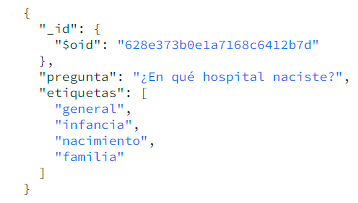
\includegraphics[scale=1.3]{Imagenes/Vectorial/mongo_pregunta}
	\caption{Documento de la colección de preguntas}
	\label{fig:mongo_preg}
\end{figure}

Por otro lado, la colección de respuestas contiene la información relativa a lo que ha respondido un usuario específico a una pregunta concreta. Es por eso, que el usuario que ha contestado y la pregunta respondida deben ser campos de esta colección. A continuación se explica cada uno de los campos:

\begin{itemize}
	\item ``user\_id'': Para distinguir al usuario se almacena el identificador que le corresponde una vez registrado en la página web. Los detalles de la aplicación web se explicarán en el capítulo siguiente. Sin embargo, para poder entender de dónde se extrae ese identificador, se explicará brevemente en que consiste. Diferentes usuarios pueden acceder al Chatbot desde la aplicación y para poder distinguir la información que se recopila es necesario tener un control de usuarios. Se crea una tabla en MySQL con todos los usuarios que se van registrando ya a cada uno se le asigna un identificador. Este identificador es el que se va a guardar en la colección de respuestas para poder diferenciar las contestaciones que da cada usuario desde la página del Chatbot. En un principio, cuando la aplicación web no se había creado, no era necesaria la distinción de usuarios porque solo se invocaba al chatbot desde un único terminal asociado a una única persona. Es decir, las respuestas se podían almacenar suponiendo que siempre respondía la misma persona. No obstante, esta solución pierde escalabilidad. 
	\item ``pregunta'': Se corresponde con la pregunta que ha elegido el Chatbot para lanzar al usuario. Coincidiría con una de las muchas que están almacenadas en la colección de preguntas que se ha explicado anteriormente. 
	\item ``respuesta'': La contestación textual que ha dado el usuario a la pregunta formulada por el bot. 
	\item ``categorias'': Una serie de características que explican la respuesta. Entre ellas se encuentra la etapa de vida en la que puede encajarse el recuerdo y el resultado del análisis de sentimiento al que se le ha sometido en forma de ``positivo'' o ``negativo'' según las connotaciones reconocidas. Además, se almacenan los lemas extraídos mediante el procesamiento léxico que se ha explicado en la sección anterior. Se trata de los lemas de aquellas palabras del texto que no sean vacías y que definen a la contestación recibida. Se consigue un desglose y un análisis bastante exhaustivo de cada respuesta. 
\end{itemize}

En la figura \ref{fig:mongo_resp} se muestra un ejemplo de documento de la colección de respuestas.

\begin{figure}[h]
	\centering
	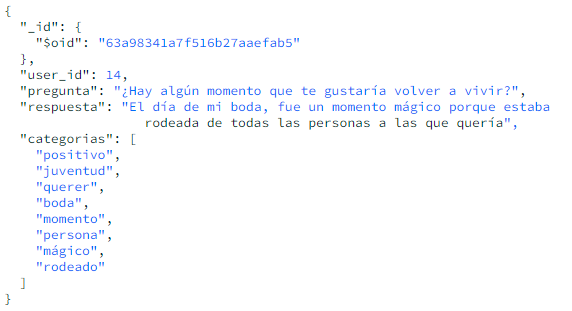
\includegraphics[scale=1.0]{Imagenes/Vectorial/mongo_respuesta}
	\caption{Documento de la colección de respuestas}
	\label{fig:mongo_resp}
\end{figure}



%\include{Capitulos/Capitulo4}
%\include{Capitulos/Capitulo5}
\chapter{Conclusiones y Trabajo Futuro}
\label{cap:conclusiones}

Conclusiones del trabajo y líneas de trabajo futuro.


Mejorar el analisis de sentimiento, mejorar la clasificación ene etapas de vida que funciona fatal y añadirle más inteligencia la chatbol con mayor precision y fluidez de conversación entre preguntas y respuestas. Que no solo conteste con una pregunta sino que reaccione a los mensajes del paciente añadiendo algún modulo de mensajería. Mejorar la aplicacion web para que el terapeuta tenga mas funcionalidades como la de poder añadir las tematicas que quiera trara con el paciente o preguntas que uiera proponer para el chatbot.

%%%%%%%%%%%%%%%%%%%%%%%%%%%%%%%%%%%%%%%%%%%%%%%%%%%%%%%%%%%%%%%%%%%%%%%%%%%
% Si el TFM se escribe en inglés, comentar las siguientes líneas 
% porque no es necesario incluir nuevamente las Conclusiones en inglés
\setcounter{chapter}{\thechapter-1} 
\begin{otherlanguage}{english}
\chapter{Conclusions and Future Work}
\label{cap:conclusions}

The aim of this TFG was to build a Chatbot intelligent enough to collect information about the life of a person with dementia and store it in a structured way. Although there is still a lot of work to be done on what has already been developed, a functional application has been built that serves as a relatively autonomous support tool in the hard task of writing a life story.

Initially, the idea was to develop a conversational bot with which a sophisticated and coherent conversation could be held. As time went by, as we encountered numerous obstacles and saw the complexity of simulating a therapist's interview, the initial idea was distorted a little.In the end, a useful tool has been created because it fulfils the function of collecting the information provided by the user, although it is not as intelligent as initially proposed, especially when it comes to giving it the human touch. It lacks the capacity to help the person with dementia to remember through stimuli and a fluid conversation.

In any case, a pretty precise analysis of the answers given by the user through the chat has been achieved. The tool manages to structure memories into the stages of the person's life to which they correspond in a fairly exact way, as happens with the sentiment analysis of the texts. Although a more concrete distinction could be made, especially in the case of memories that do not fall into any of the categories provided, it is left as a possible future work. This is because for the technologies used, the volume of data was quite small, and would have worked better with a much larger dataset of memories. On another note, the conversation is made more fluid by the answer and question chaining module that analyses the user's answer to find the best next question to ask. Further analysis of the context of the sentence would have greatly improved the choice of coherent and fluid questions.

At the web application level, it is quite manageable and interactive, offering a user-friendly interface aimed at both patients and therapists. It offers control over the users and over the information that is collected. More functionalities have not been added because the focus should be the Chatbot and, in addition, there were already other works (TFGs) that focused on a more specific web development.

In terms of future work, the following improvements are proposed:

\begin{itemize}
	\item More accurate and concrete sentiment analysis and life-stage classification. An improvement of this analysis by using a much larger memory dataset to train the model.
	\item A more fluid conversation with the user: apart from asking about their past, implement a conversational module that simply reacts to the answers, always according to what the person has said. Also include a program to complete the missing information about the user according to a template to be filled in.
	\item Add some extra functionality to the web application such as defining specific therapies aimed at a specific topic. Other functionalities could be allowing the therapist to add questions to the battery available in the database, enabling a voice recognition option to make it much easier for the dementia patient to interact with the Chatbot, etc.
	\item A better choice of the questions posed to the user: apart from comparing the answer given by the user to choose the next question, also compare with the question that was asked to which the user answered. For example, if a question has been asked about something related to childhood, keep asking about things related to childhood. Ontologies can also be implemented so that when analysing the answers, words or concepts can be related to new possible questions to be asked.
	\item Expand the battery of questions and topics to be addressed by adapting the standard interviews conducted by occupational therapists.
	\item Create the possibility that questions can be generated on their own, without being previously drafted, according to the topic being dealt with and the data provided by the patient.
	\item Greater categorisation of memories with labels such as family, friends, leisure, food, holidays, hobbies, etc.
\end{itemize}















\end{otherlanguage}
%%%%%%%%%%%%%%%%%%%%%%%%%%%%%%%%%%%%%%%%%%%%%%%%%%%%%%%%%%%%%%%%%%%%%%%%%%%


% Apéndices
\appendix
%\chapter{Título}
\label{Appendix:Key1}

Contenido del apéndice
%\chapter{Título}
\label{Appendix:Key2}

%\include{Apendices/appendixC}
%\include{...}
%\include{...}
%\include{...}
\backmatter

%
% Bibliografía
%
% Si el TFM se escribe en inglés, editar TeXiS/TeXiS_bib para cambiar el
% estilo de las referencias
%---------------------------------------------------------------------
%
%                      configBibliografia.tex
%
%---------------------------------------------------------------------
%
% bibliografia.tex
% Copyright 2009 Marco Antonio Gomez-Martin, Pedro Pablo Gomez-Martin
%
% This file belongs to the TeXiS manual, a LaTeX template for writting
% Thesis and other documents. The complete last TeXiS package can
% be obtained from http://gaia.fdi.ucm.es/projects/texis/
%
% Although the TeXiS template itself is distributed under the 
% conditions of the LaTeX Project Public License
% (http://www.latex-project.org/lppl.txt), the manual content
% uses the CC-BY-SA license that stays that you are free:
%
%    - to share & to copy, distribute and transmit the work
%    - to remix and to adapt the work
%
% under the following conditions:
%
%    - Attribution: you must attribute the work in the manner
%      specified by the author or licensor (but not in any way that
%      suggests that they endorse you or your use of the work).
%    - Share Alike: if you alter, transform, or build upon this
%      work, you may distribute the resulting work only under the
%      same, similar or a compatible license.
%
% The complete license is available in
% http://creativecommons.org/licenses/by-sa/3.0/legalcode
%
%---------------------------------------------------------------------
%
% Fichero  que  configura  los  parámetros  de  la  generación  de  la
% bibliografía.  Existen dos  parámetros configurables:  los ficheros
% .bib que se utilizan y la frase célebre que aparece justo antes de la
% primera referencia.
%
%---------------------------------------------------------------------


%%%%%%%%%%%%%%%%%%%%%%%%%%%%%%%%%%%%%%%%%%%%%%%%%%%%%%%%%%%%%%%%%%%%%%
% Definición de los ficheros .bib utilizados:
% \setBibFiles{<lista ficheros sin extension, separados por comas>}
% Nota:
% Es IMPORTANTE que los ficheros estén en la misma línea que
% el comando \setBibFiles. Si se desea utilizar varias líneas,
% terminarlas con una apertura de comentario.
%%%%%%%%%%%%%%%%%%%%%%%%%%%%%%%%%%%%%%%%%%%%%%%%%%%%%%%%%%%%%%%%%%%%%%
\setBibFiles{%
nuestros,latex,otros%
}

%%%%%%%%%%%%%%%%%%%%%%%%%%%%%%%%%%%%%%%%%%%%%%%%%%%%%%%%%%%%%%%%%%%%%%
% Definición de la frase célebre para el capítulo de la
% bibliografía. Dentro normalmente se querrá hacer uso del entorno
% \begin{FraseCelebre}, que contendrá a su vez otros dos entornos,
% un \begin{Frase} y un \begin{Fuente}.
%
% Nota:
% Si no se quiere cita, se puede eliminar su definición (en la
% macro setCitaBibliografia{} ).
%%%%%%%%%%%%%%%%%%%%%%%%%%%%%%%%%%%%%%%%%%%%%%%%%%%%%%%%%%%%%%%%%%%%%%
\setCitaBibliografia{
\begin{FraseCelebre}
\begin{Frase}
  Y así, del mucho leer y del poco dormir, se le secó el celebro de
  manera que vino a perder el juicio.
\end{Frase}
\begin{Fuente}
  Miguel de Cervantes Saavedra
\end{Fuente}
\end{FraseCelebre}
}

%%
%% Creamos la bibliografia
%%
\makeBib


% Variable local para emacs, para  que encuentre el fichero maestro de
% compilación y funcionen mejor algunas teclas rápidas de AucTeX

%%%
%%% Local Variables:
%%% mode: latex
%%% TeX-master: "../Tesis.tex"
%%% End:

%
% Índice de palabras
%

% Sólo  la   generamos  si  está   declarada  \generaindice.  Consulta
% TeXiS.sty para más información.

% En realidad, el soporte para la generación de índices de palabras
% en TeXiS no está documentada en el manual, porque no ha sido usada
% "en producción". Por tanto, el fichero que genera el índice
% *no* se incluye aquí (está comentado). Consulta la documentación
% en TeXiS_pream.tex para más información.
\ifx\generaindice\undefined
\else
%%---------------------------------------------------------------------
%
%                        TeXiS_indice.tex
%
%---------------------------------------------------------------------
%
% TeXiS_indice.tex
% Copyright 2009 Marco Antonio Gomez-Martin, Pedro Pablo Gomez-Martin
%
% This file belongs to TeXiS, a LaTeX template for writting
% Thesis and other documents. The complete last TeXiS package can
% be obtained from http://gaia.fdi.ucm.es/projects/texis/
%
% This work may be distributed and/or modified under the
% conditions of the LaTeX Project Public License, either version 1.3
% of this license or (at your option) any later version.
% The latest version of this license is in
%   http://www.latex-project.org/lppl.txt
% and version 1.3 or later is part of all distributions of LaTeX
% version 2005/12/01 or later.
%
% This work has the LPPL maintenance status `maintained'.
% 
% The Current Maintainers of this work are Marco Antonio Gomez-Martin
% and Pedro Pablo Gomez-Martin
%
%---------------------------------------------------------------------
%
% Contiene  los  comandos  para  generar  el índice  de  palabras  del
% documento.
%
%---------------------------------------------------------------------
%
% NOTA IMPORTANTE: el  soporte en TeXiS para el  índice de palabras es
% embrionario, y  de hecho  ni siquiera se  describe en el  manual. Se
% proporciona  una infraestructura  básica (sin  terminar)  para ello,
% pero  no ha  sido usada  "en producción".  De hecho,  a pesar  de la
% existencia de  este fichero, *no* se incluye  en Tesis.tex. Consulta
% la documentación en TeXiS_pream.tex para más información.
%
%---------------------------------------------------------------------


% Si se  va a generar  la tabla de  contenidos (el índice  habitual) y
% también vamos a  generar el índice de palabras  (ambas decisiones se
% toman en  función de  la definición  o no de  un par  de constantes,
% puedes consultar modo.tex para más información), entonces metemos en
% la tabla de contenidos una  entrada para marcar la página donde está
% el índice de palabras.

\ifx\generatoc\undefined
\else
   \addcontentsline{toc}{chapter}{\indexname}
\fi


% Generamos el índice
\printindex

% Variable local para emacs, para  que encuentre el fichero maestro de
% compilación y funcionen mejor algunas teclas rápidas de AucTeX

%%%
%%% Local Variables:
%%% mode: latex
%%% TeX-master: "./tesis.tex"
%%% End:

\fi

%
% Lista de acrónimos
%

% Sólo  lo  generamos  si  está declarada  \generaacronimos.  Consulta
% TeXiS.sty para más información.


\ifx\generaacronimos\undefined
\else
%---------------------------------------------------------------------
%
%                        TeXiS_acron.tex
%
%---------------------------------------------------------------------
%
% TeXiS_acron.tex
% Copyright 2009 Marco Antonio Gomez-Martin, Pedro Pablo Gomez-Martin
%
% This file belongs to TeXiS, a LaTeX template for writting
% Thesis and other documents. The complete last TeXiS package can
% be obtained from http://gaia.fdi.ucm.es/projects/texis/
%
% This work may be distributed and/or modified under the
% conditions of the LaTeX Project Public License, either version 1.3
% of this license or (at your option) any later version.
% The latest version of this license is in
%   http://www.latex-project.org/lppl.txt
% and version 1.3 or later is part of all distributions of LaTeX
% version 2005/12/01 or later.
%
% This work has the LPPL maintenance status `maintained'.
% 
% The Current Maintainers of this work are Marco Antonio Gomez-Martin
% and Pedro Pablo Gomez-Martin
%
%---------------------------------------------------------------------
%
% Contiene  los  comandos  para  generar  el listado de acrónimos
% documento.
%
%---------------------------------------------------------------------
%
% NOTA IMPORTANTE:  para que la  generación de acrónimos  funcione, al
% menos  debe  existir  un  acrónimo   en  el  documento.  Si  no,  la
% compilación  del   fichero  LaTeX  falla  con   un  error  "extraño"
% (indicando  que  quizá  falte  un \item).   Consulta  el  comentario
% referente al paquete glosstex en TeXiS_pream.tex.
%
%---------------------------------------------------------------------


% Redefinimos a español  el título de la lista  de acrónimos (Babel no
% lo hace por nosotros esta vez)

\def\listacronymname{Lista de acrónimos}

% Para el glosario:
% \def\glosarryname{Glosario}

% Si se  va a generar  la tabla de  contenidos (el índice  habitual) y
% también vamos a  generar la lista de acrónimos  (ambas decisiones se
% toman en  función de  la definición  o no de  un par  de constantes,
% puedes consultar config.tex  para más información), entonces metemos
% en la  tabla de contenidos una  entrada para marcar  la página donde
% está el índice de palabras.

\ifx\generatoc\undefined
\else
   \addcontentsline{toc}{chapter}{\listacronymname}
\fi


% Generamos la lista de acrónimos (en realidad el índice asociado a la
% lista "acr" de GlossTeX)

\printglosstex(acr)

% Variable local para emacs, para  que encuentre el fichero maestro de
% compilación y funcionen mejor algunas teclas rápidas de AucTeX

%%%
%%% Local Variables:
%%% mode: latex
%%% TeX-master: "../Tesis.tex"
%%% End:

\fi

%
% Final
%
%\end{otherlanguage}
\end{document}
